\section{1-DOF System}
We consider as transfer function from voltage to the mass speed:\\
\\
\[	
G(s)=
\frac{-5.618*10^{4}}{{s^3+21.45*s^{2}}+1699*s+3.149*10^{4}}
\]
\\


\begin{figure*}[h]
	\centering
	\begin{subfigure}{0.4\columnwidth}
		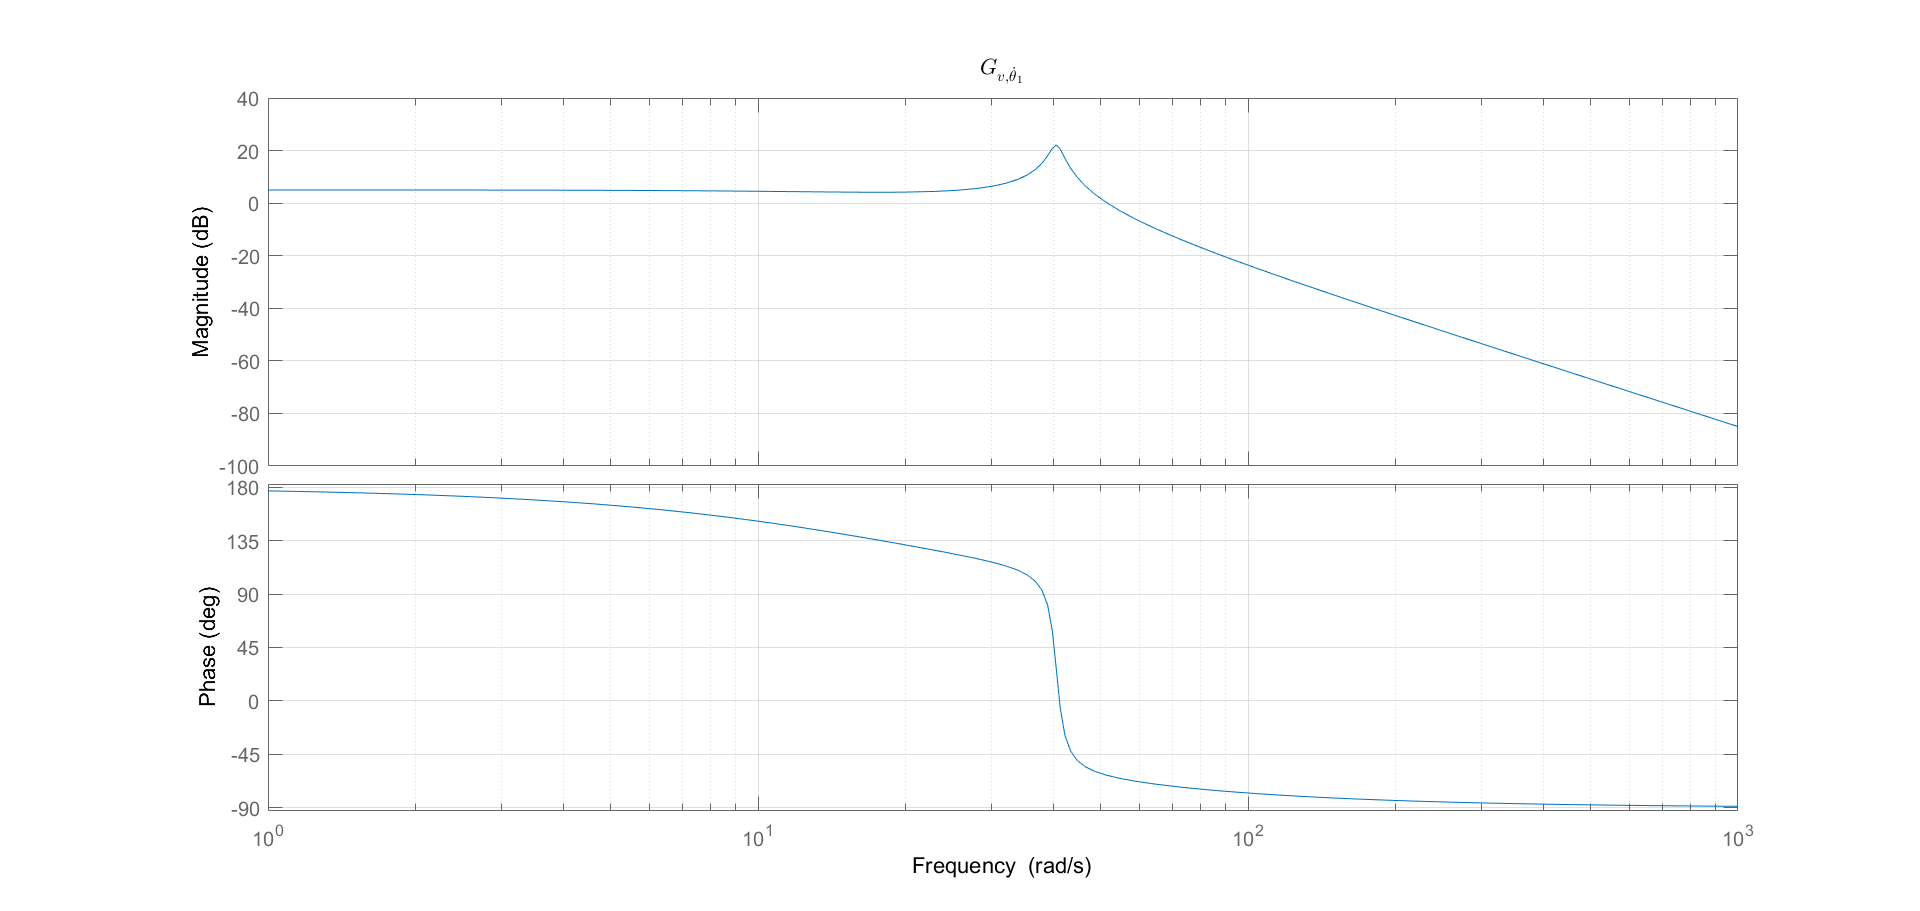
\includegraphics[width=\textwidth]{1Bode_G}
	\end{subfigure}
	\begin{subfigure}{0.4\columnwidth}
		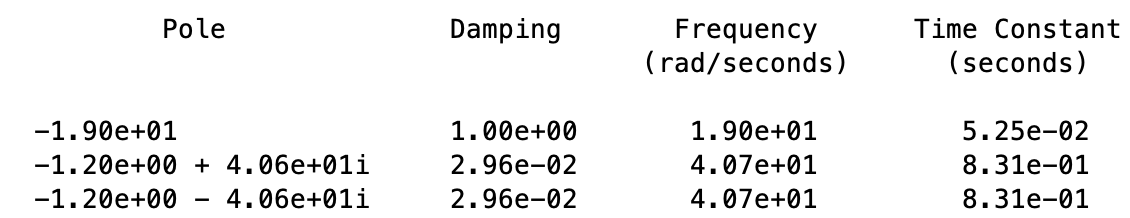
\includegraphics[width=\textwidth]{1Pole_G}
	\end{subfigure}
	\caption{G(s)}
	\label{fig:G(s)1dof}
\end{figure*}

As it is possible to notice in figure \ref{fig:G(s)1dof}, there is a couple of complex conjugated poles with low damping coefficient. We decide so to apply a notch filter, thanks to which we are able to delete these poles and substitute them with a couple of complex conjugated poles at the same frequency but with a damping coefficent equal to 0.72. We decide not to alter too much the behavior of the plant not to have a too aggressive control action, for this reason we do not impose real poles or high frequency poles.

\begin{figure*}[h]
	\centering
	\begin{subfigure}{0.35\columnwidth}
		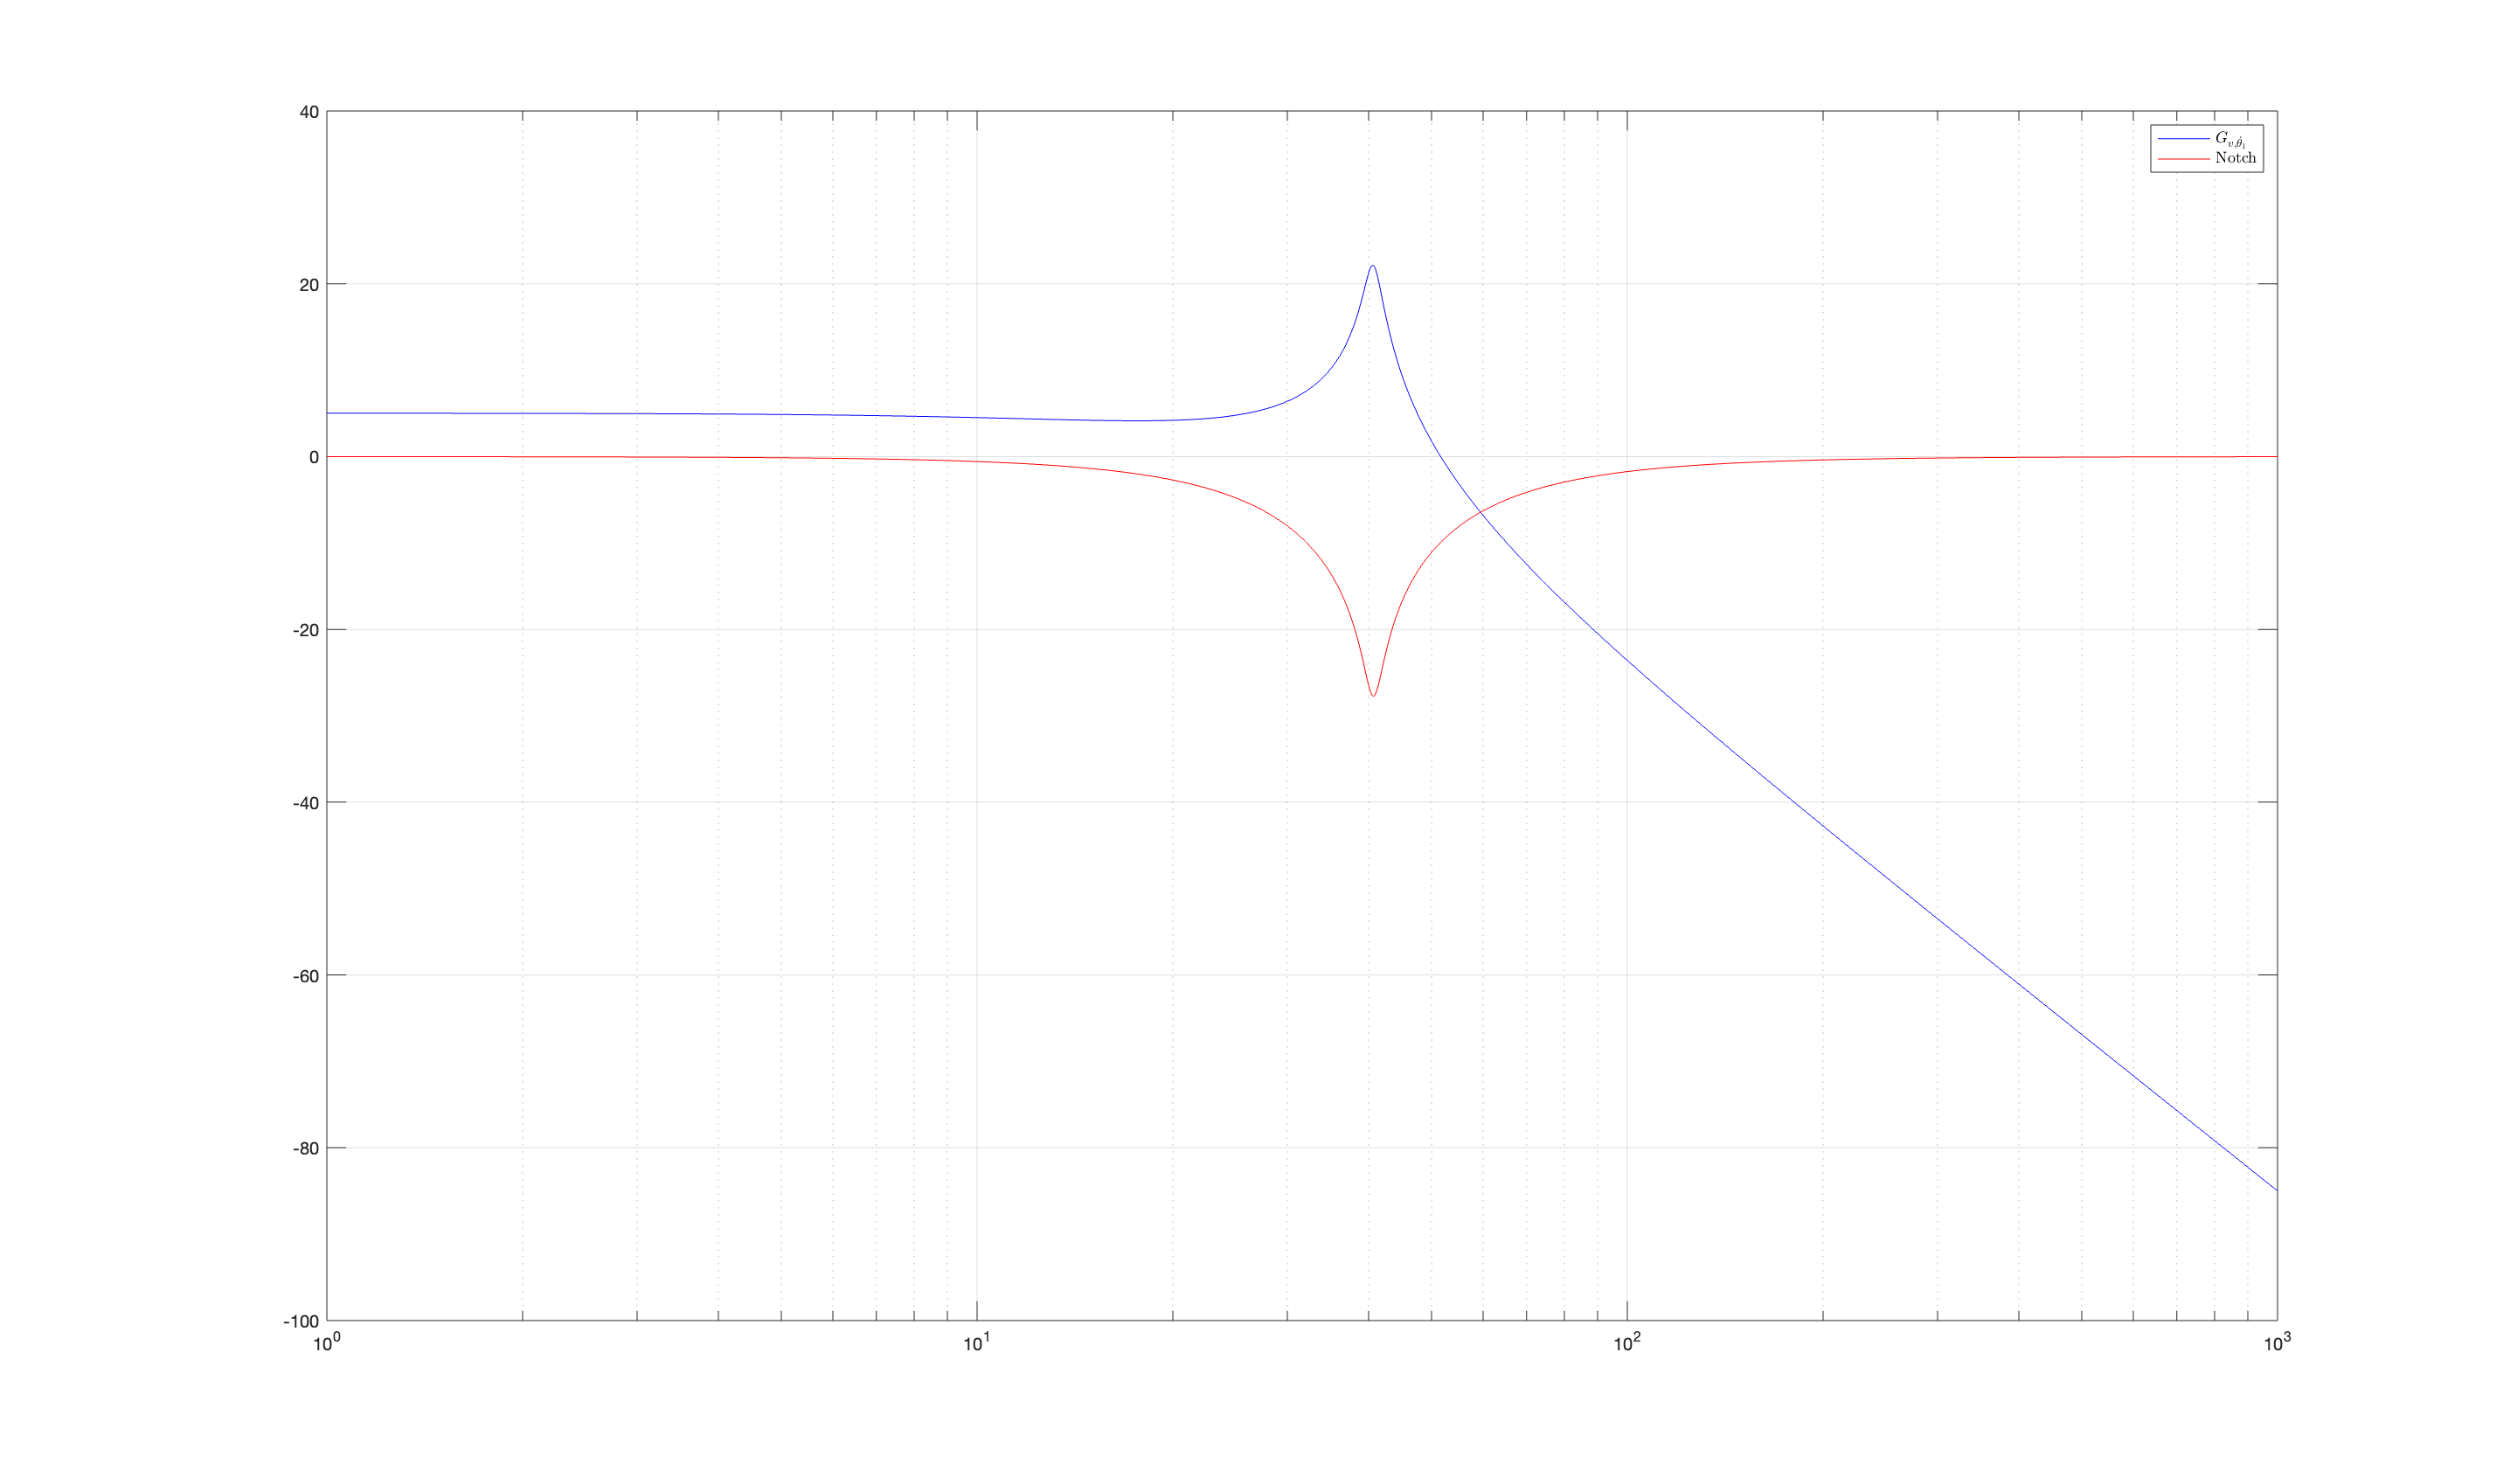
\includegraphics[width=\textwidth]{1Nf_G}
		\subcaption{Nf(s) and G(s)}
	\end{subfigure}
	\begin{subfigure}{0.35\columnwidth}
		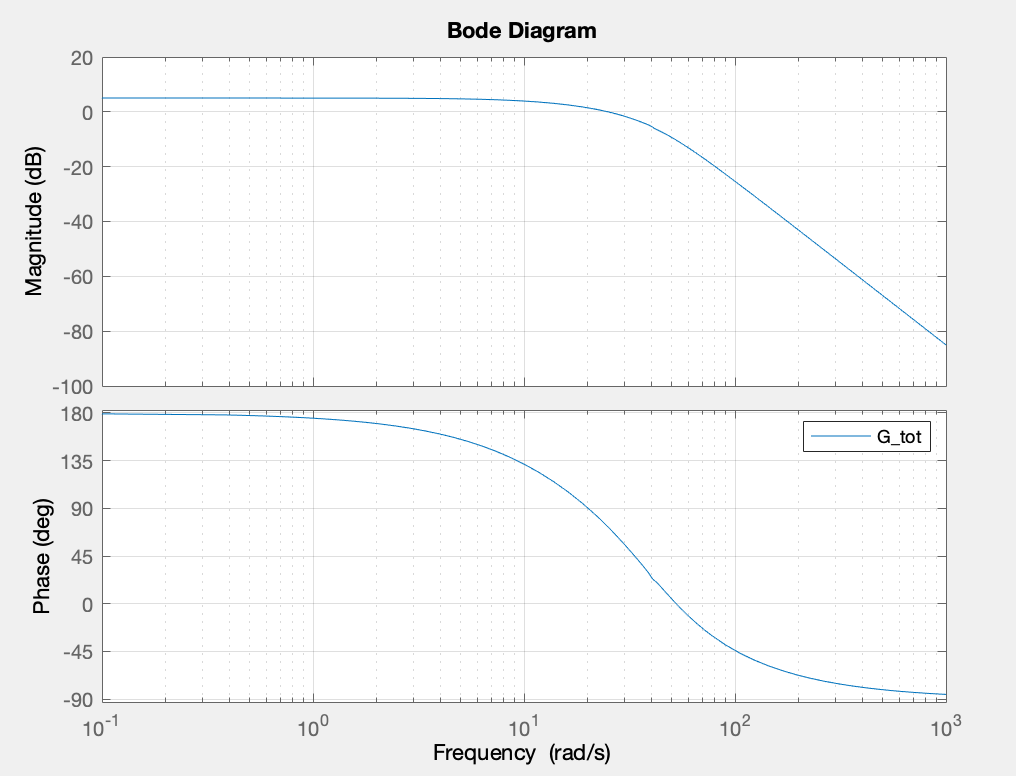
\includegraphics[width=\textwidth]{1_Gtot}
		\subcaption{$G_{tot}$(s)}
	\end{subfigure}
	\caption{Plant G(s) with Notch Filter Nf(s): $G_{tot}$(s)}
	\label{fig:Plant G(s)with Notch Filter1}
\end{figure*}


Applying the notch filter represented in figure \ref{fig:Plant G(s)with Notch Filter1}(a), we obtain the plant $G_{tot}$(s) of figure \ref{fig:Plant G(s)with Notch Filter1}(b) that is the system we are going to control.



\newpage
\subsection{Speed Control Loop}
We choose as regulator the PI controller enriched with an anti-windup structure, with which we cancel out the real frequency pole at 19 rad/s. \\
\\
\[
R(s)=-wc_v
\frac{\frac{s}{19}+1}{s}
\]
\\

We would like to have a cutting frequency at 10 rad/s,but we notice that, due to the presence of the notch-filter, the cutting frequency imposed by the PI-controller is postponed. For this reason, from now on we will use $wc_v$ only as the parameter set inside of the PI regulator and not to define the real bandwidth of the speed loop.
\\
\begin{figure*}[h]
	\centering
	\begin{subfigure}{0.45\columnwidth}
		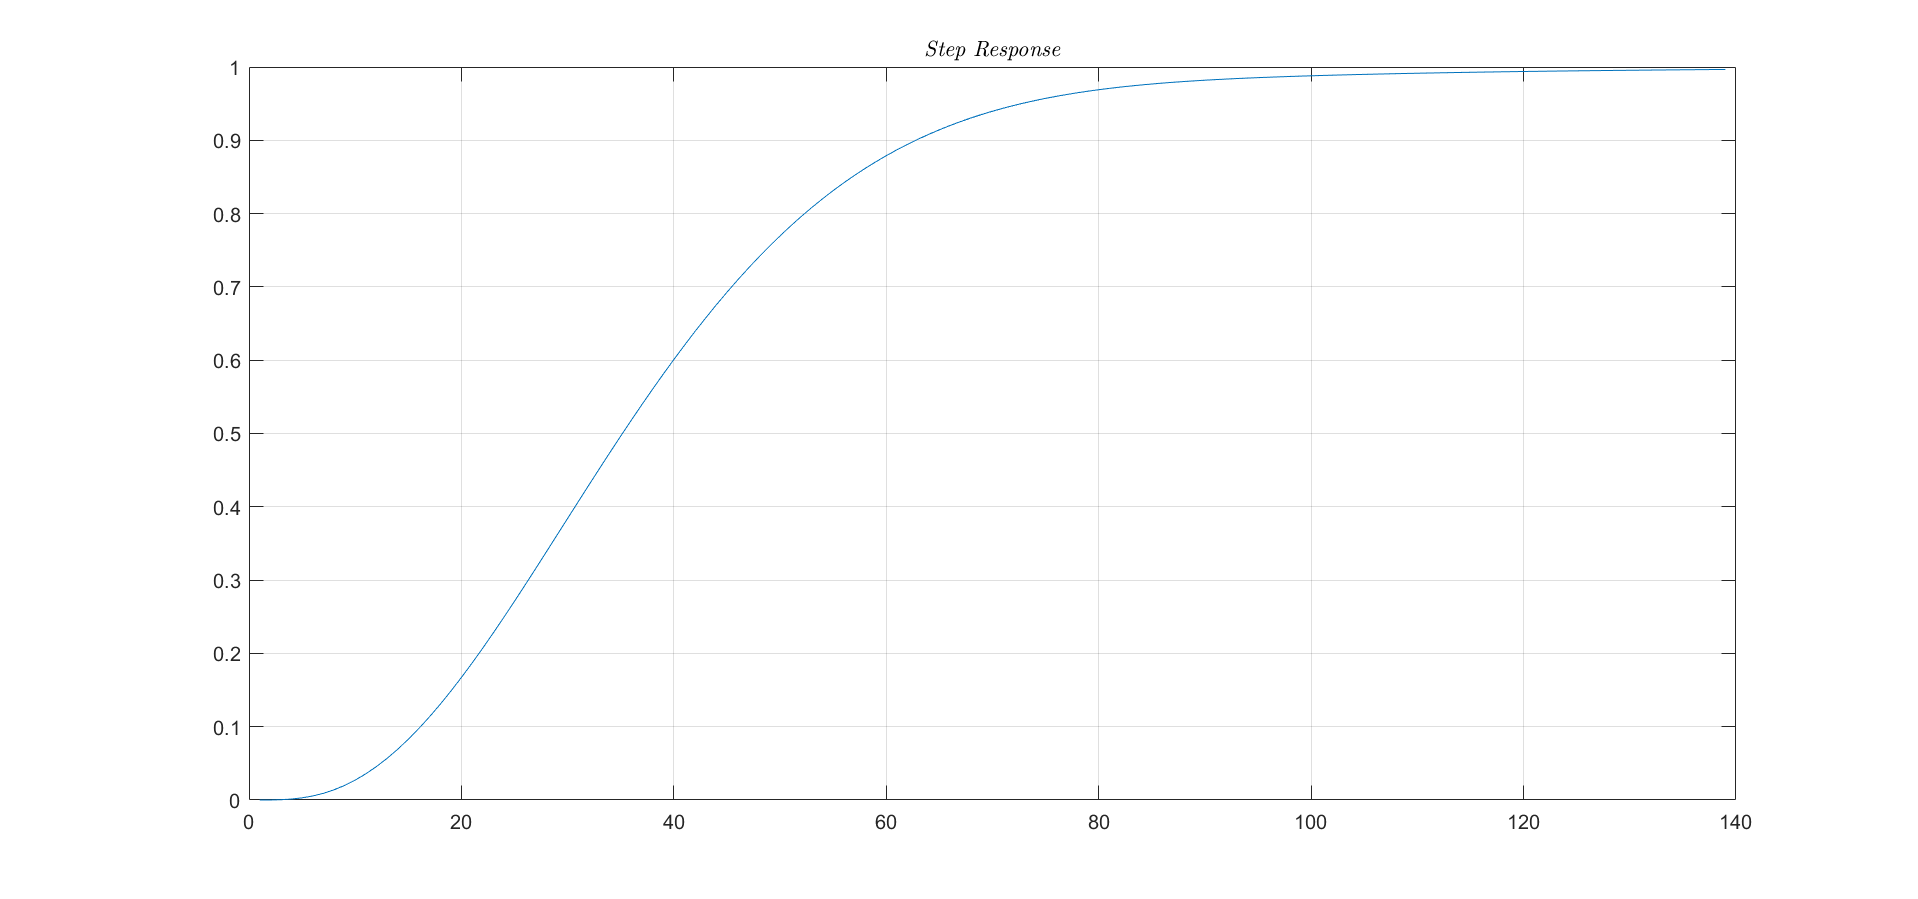
\includegraphics[width=\textwidth]{1step10}
	\end{subfigure}
	\begin{subfigure}{0.45\columnwidth}
		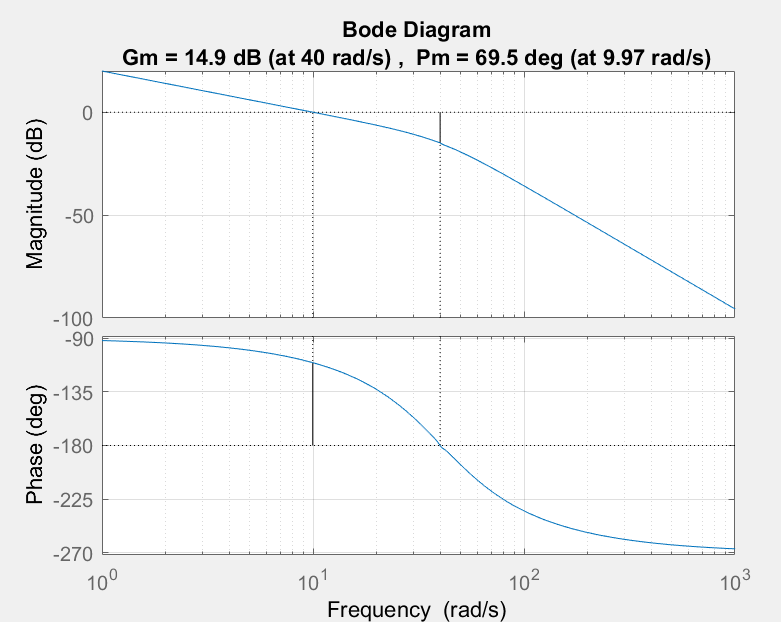
\includegraphics[width=\textwidth]{1bode10}
	\end{subfigure}
	\caption{Speed control loop with  $wc_{v} $=10 rad/s}
	\label{fig:Bode and Step PI 10}
\end{figure*}
\\
This closed loop system would lead us to the step response of the figure \ref{fig:Bode and Step PI 10}. 
Even if this response could be considered acceptable, we have to remember that this is just a simulation. Having such a low phase margin might generate undesidered behavior in presence of disturbance of the real system. In order to have a more robust control system, it is so necessary to increase the phase margin by reducing the cutting frequency. 
\newline After many tests at the laboratory we choose for the best configuration which is obtained by setting $wc_{v} $=4.5. We consider this solution a good trade-off between the settling time and the robustness of the closed loop system.
We consider one of the worst case scenarios, that is the step from -17 rad/s to 17 rad/s, and then we apply a step of 10 rad/s. The first one lets us to asses the voltage saturation while the second one the transient after an ordinary step.
We plot them comparing the simulation and the data collected in the laboratory.

\newpage

\begin{figure*}[h]
	\centering
	\begin{subfigure}{0.4\columnwidth}
		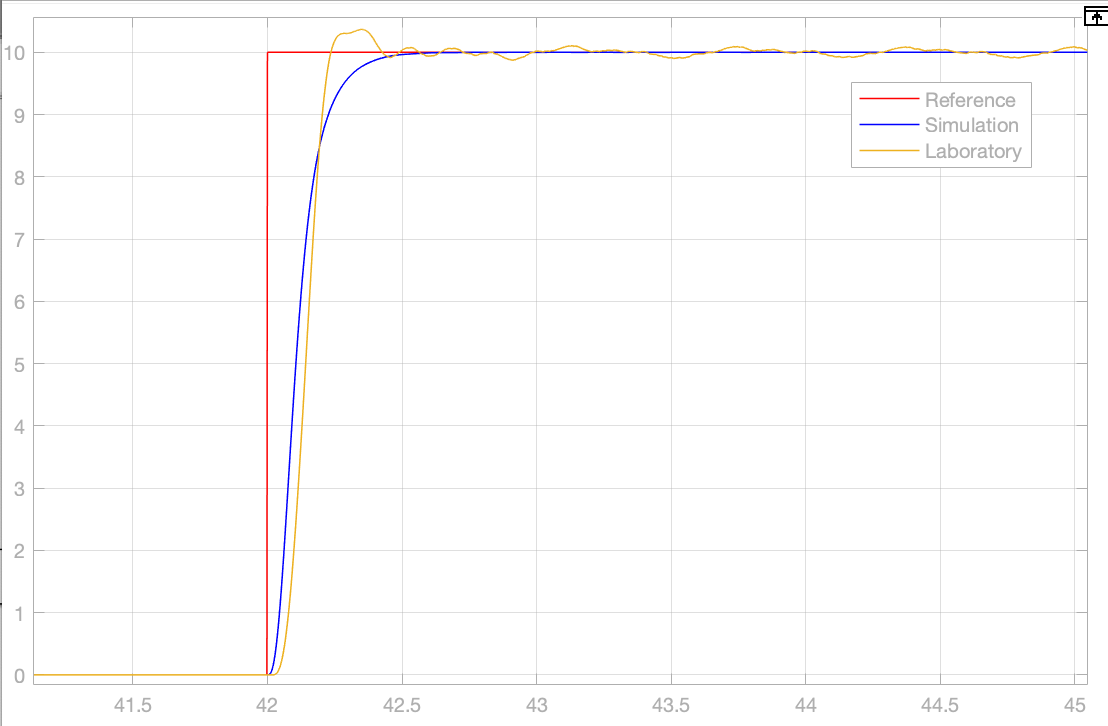
\includegraphics[width=\textwidth]{1_step10}
		\subcaption{Step 10 rad/s}
	\end{subfigure}
	\begin{subfigure}{0.4\columnwidth}
		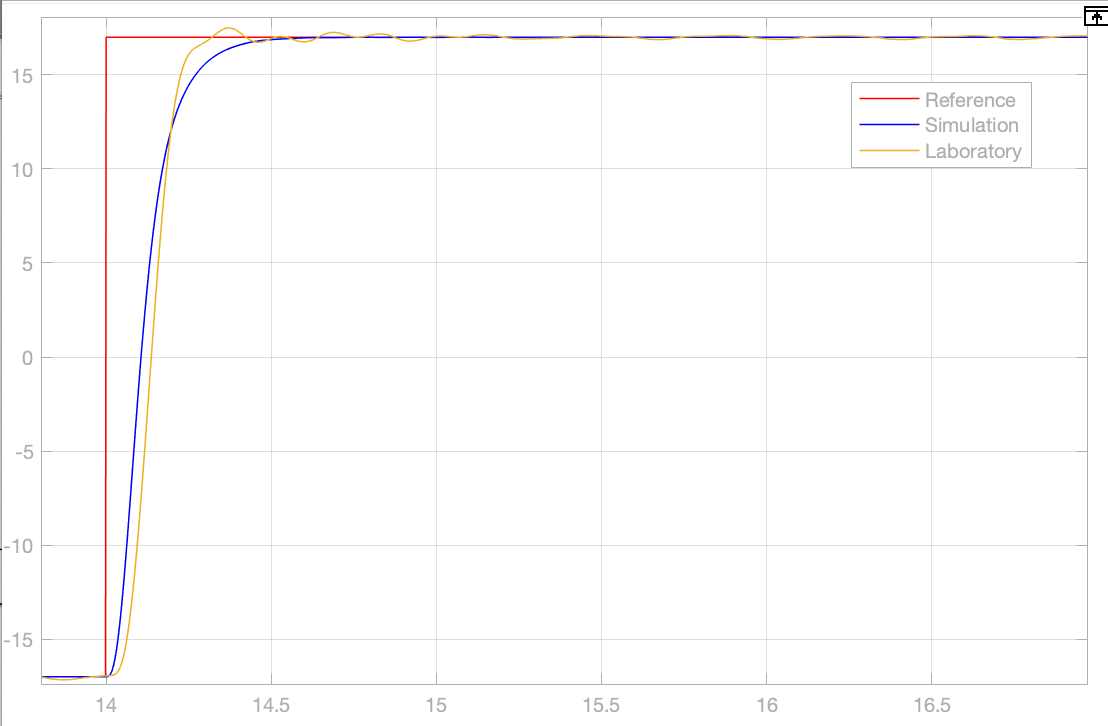
\includegraphics[width=\textwidth]{1_step17}
		\subcaption{Step 17 rad/s}
	\end{subfigure}
	\begin{subfigure}{0.4\columnwidth}
		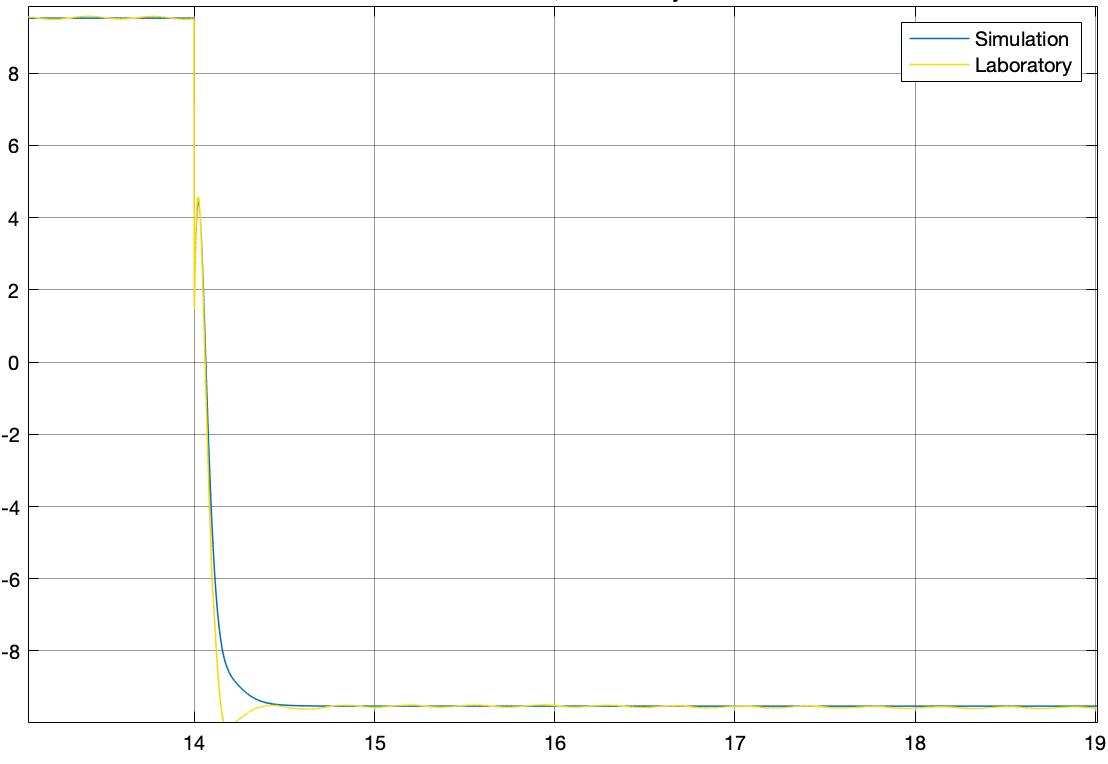
\includegraphics[width=\textwidth]{1_volt17}
		\subcaption{Voltage related to a step of 17 rad/s}
	\end{subfigure}
	\caption{Speed control loop with  $wc_{v} $=4.5 rad/s}
	\label{fig:PI with 4.5}
\end{figure*}

We plot now a sinesweep experiment thanks to which we are able to evaluate the bandwidth of the closed loop system and a ramp reference with a decreasing slope that lets us test the controllability range, especially for what concerns the low speeds. 
Analizing both the step and the sinesweep responses, respectively figure \ref{fig:PI with 4.5} and figure \ref{fig:sinesweep_PI_1dof}, we notice that our simulation does not follow exactly the laboratory data. This difference is caused by a not perfect identification of the real system. Indeed, estimating the bandwidth from the sinesweep experiment, we obtain two different crossover frequencies: our simulation at 11.3 rad/s and the laboratory data at 14.3 rad/s. We computed this values starting from the theory, for which the attenuation at the cutting frequency is -3dB. Moreover, we cannot neglet the fact we are controlling the speed, which is obtained through a derivation of the position of the encoder and so it is not fully reliable. Furthermore, we suppose that the dominant pole, which we estimated being at 19 rad/s, could lays at lower frequencies and additionally we have a small resonance uncertainty. As regards the dominant pole issue, the difference is mainly highlighted by the step response overshoot, while the resonance uncertainty is observable through the small oscillations at the end of the transient that are not well compensated by the notch filter.
Another aspect that has to be considered is the presence of very small oscillations, their frequencies are equal to the speed, so we suppose that it depends on a change of the dynamic friction coefficient value along the revolution. As a matter of fact, this undesired behaviour can be neglected, since the amplitude of the above-mentioned oscillations is very small. In the case in which we would like to attenuate them, we should increase the bandwidth of the loop to counteract them on time. By using just a PI this is not possible, because if we increase wcv, we face significant oscillations, that cannot be accepted. To avoid this behavior, we could just put a low pass prefilter on the reference signal, in this way a possible step on the speed reference would be made smoother and just small oscillations should arise. This solution will be analized with more details in the 2-DOF case, in which these oscillations at the steady state cannot be neglected.
\newpage
\begin{figure*}[h]
	\centering
	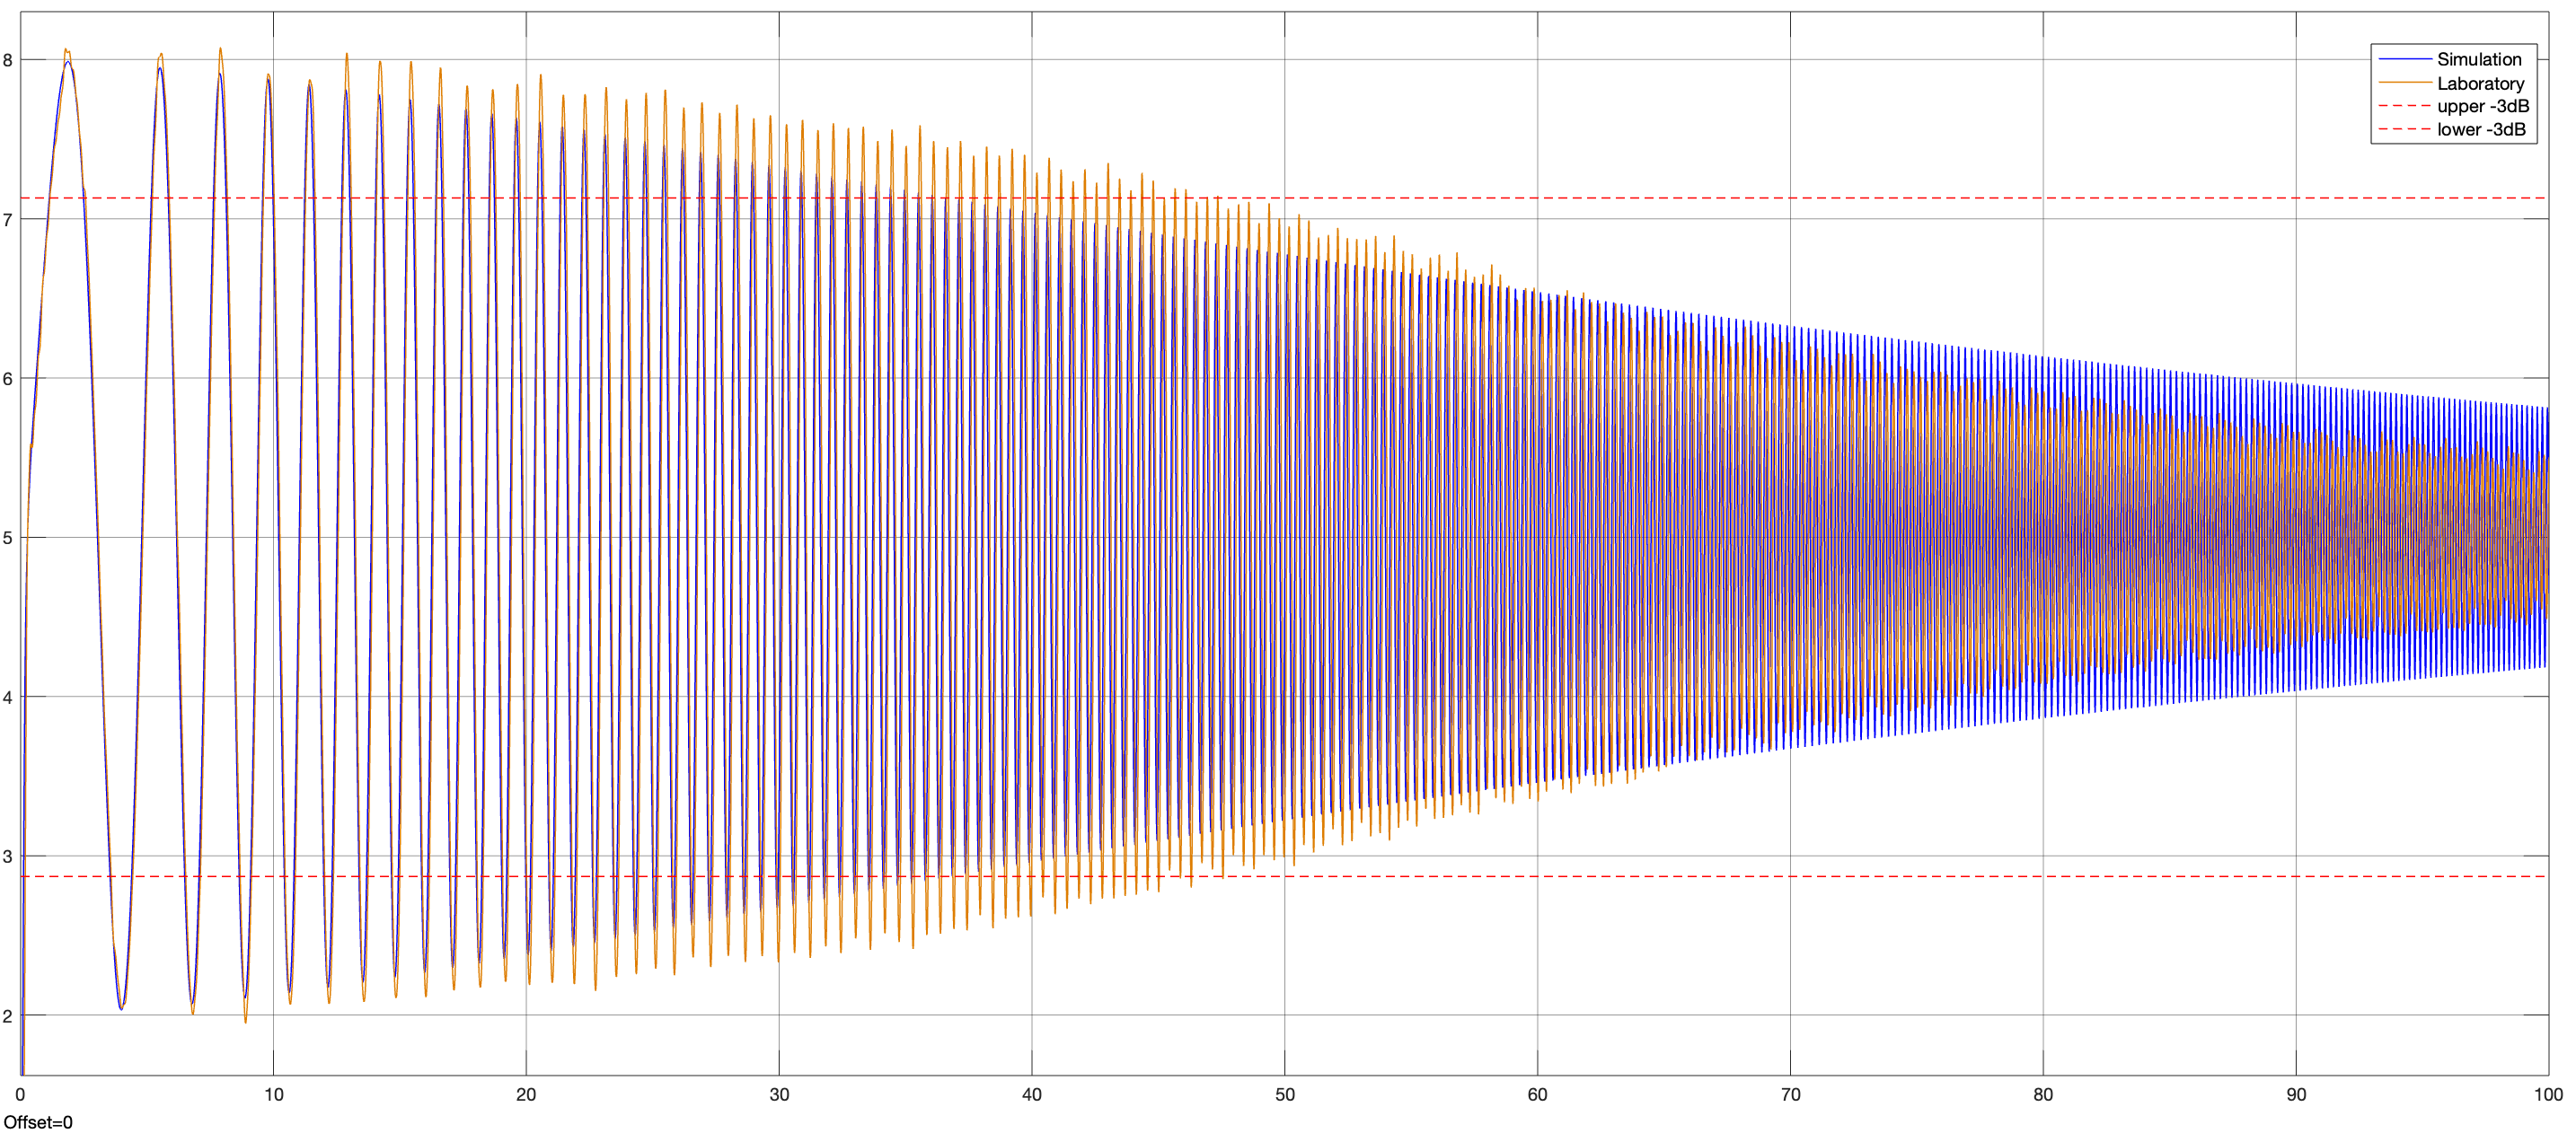
\includegraphics[scale=0.4]{Sine1dof}
	\caption{Sinesweep experiment from 0.1 Hz to 10 Hz in 100s}
	\label{fig:sinesweep_PI_1dof}
\end{figure*}

\begin{figure*}[h]
	\centering
	\begin{subfigure}{0.45\columnwidth}
		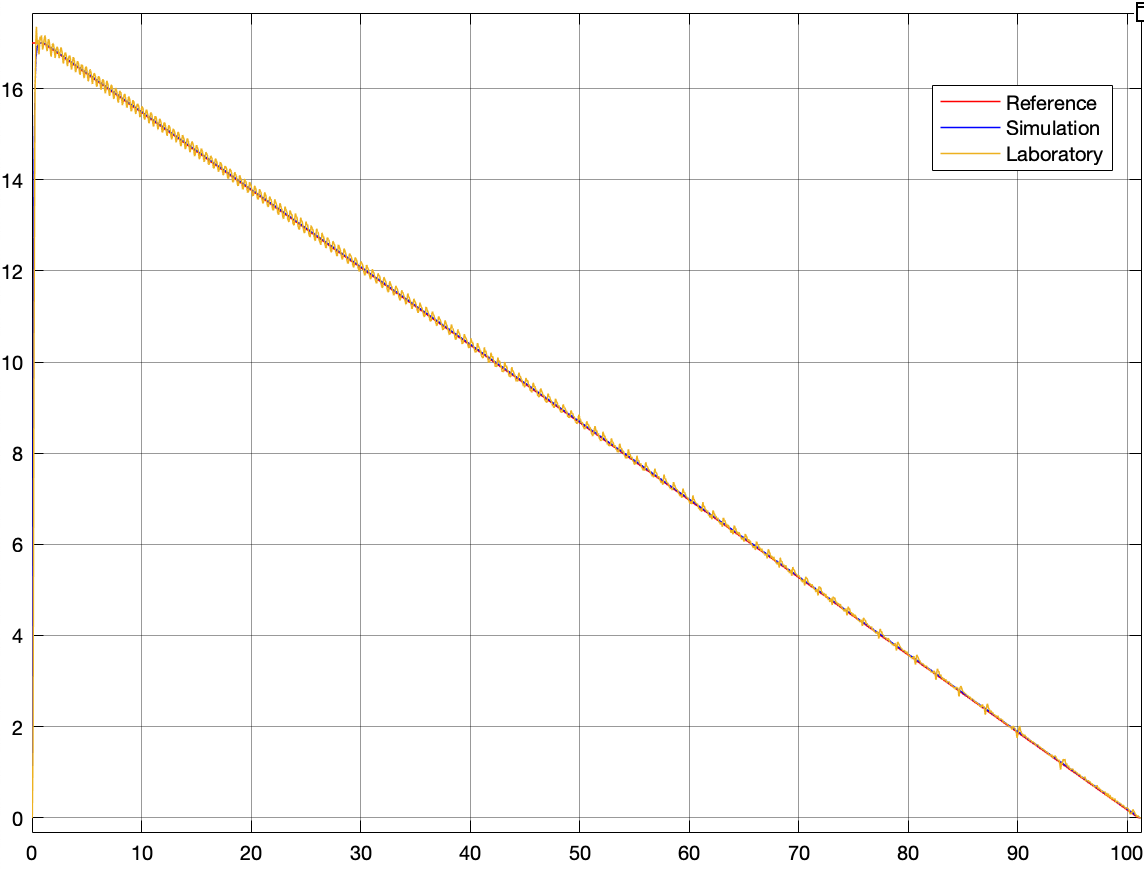
\includegraphics[width=\textwidth]{Ramp1dofa}
		\subcaption{Entire experiment}
	\end{subfigure}
	\begin{subfigure}{0.45\columnwidth}
		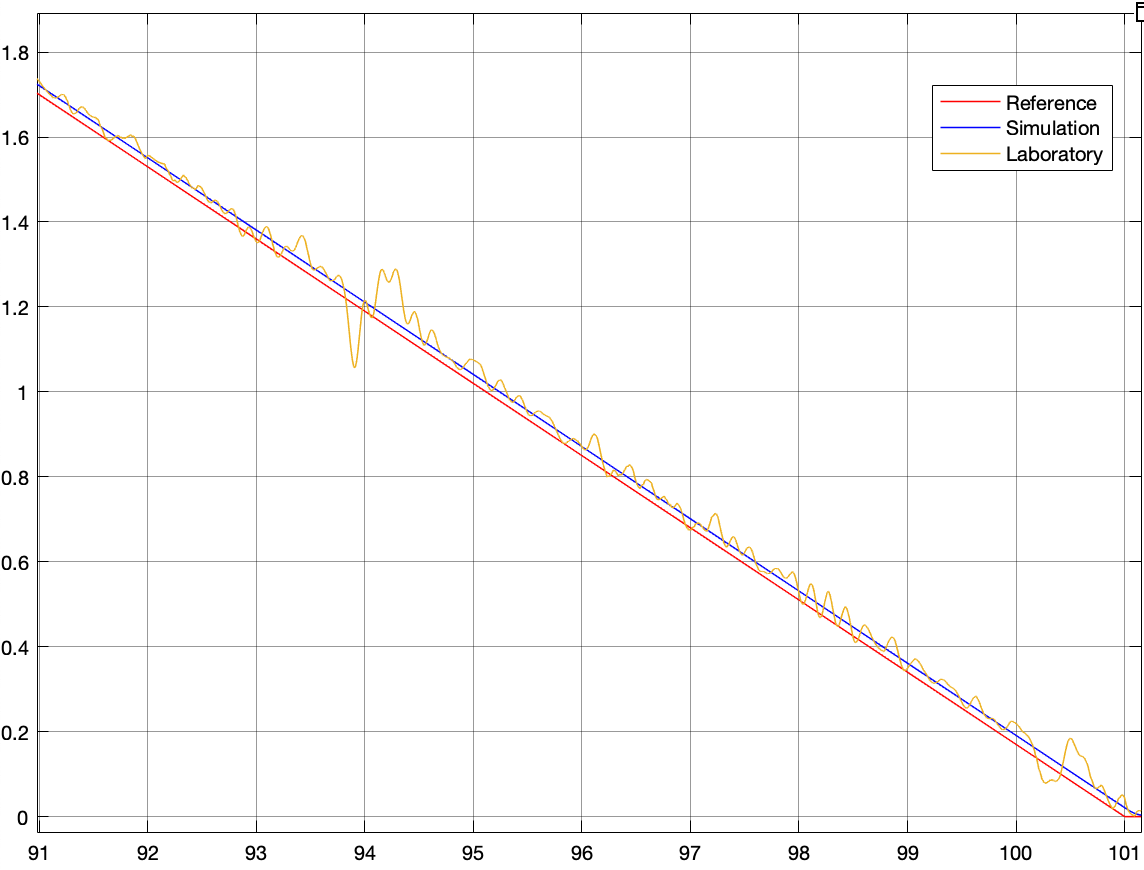
\includegraphics[width=\textwidth]{Ramp1dofb}
		\subcaption{Detail at low speed}
	\end{subfigure}
	\caption{Ramp experiment from 17 rad/s to 0 rad/s in 100s}
	\label{fig:Ramp1dof}
\end{figure*}

Thanks to the ramp experiment, we have verified that our regulator can control the system even at very low speed. This result is very satisfying, because of the wide controllability range, which goes from -17.5 rad/s to -0.3 rad/s and from 0.3 rad/s to 17.5 rad/s.

\newpage
\subsection{Position Control Loop}
To control the position, we decide to use a cascade strategy: the inner loop controls the speed, whereas the outer one the position. For the first loop we use the same PI structure as explained above, while the position is regulated by using a proportional controller. It is important to remark that the cutting frequency of the position and the speed one must be far enough (about one decade) to assure the frequency decoupling of the two loops. As consequence if we maintain the cutting frequency of the speed loop as decided before ($wc_v$=4.5 rad/s that corresponds to a bandwidth of 14.3 rad/s, as estimated in the sinesweep in figure \ref{fig:sinesweep_PI_1dof}), a first possible solution is reached by setting the position cutting frequency equal to 1.4 rad/s. This case is represented in the figure \ref{fig:Bode and Step P 1.4}. From these plots we can see that the overall system is very robust but also very slow.

\begin{figure*}[h]
	\centering
	\begin{subfigure}{0.45\columnwidth}
		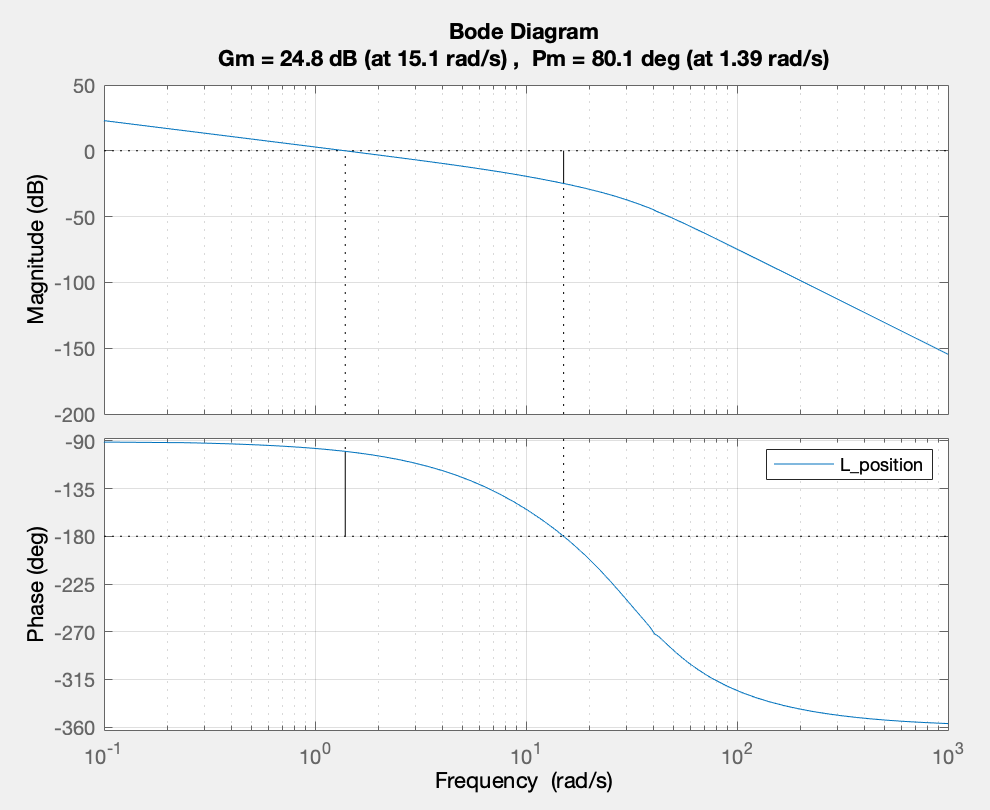
\includegraphics[width=\textwidth]{1_bode1.4}
	\end{subfigure}
	\begin{subfigure}{0.45\columnwidth}
		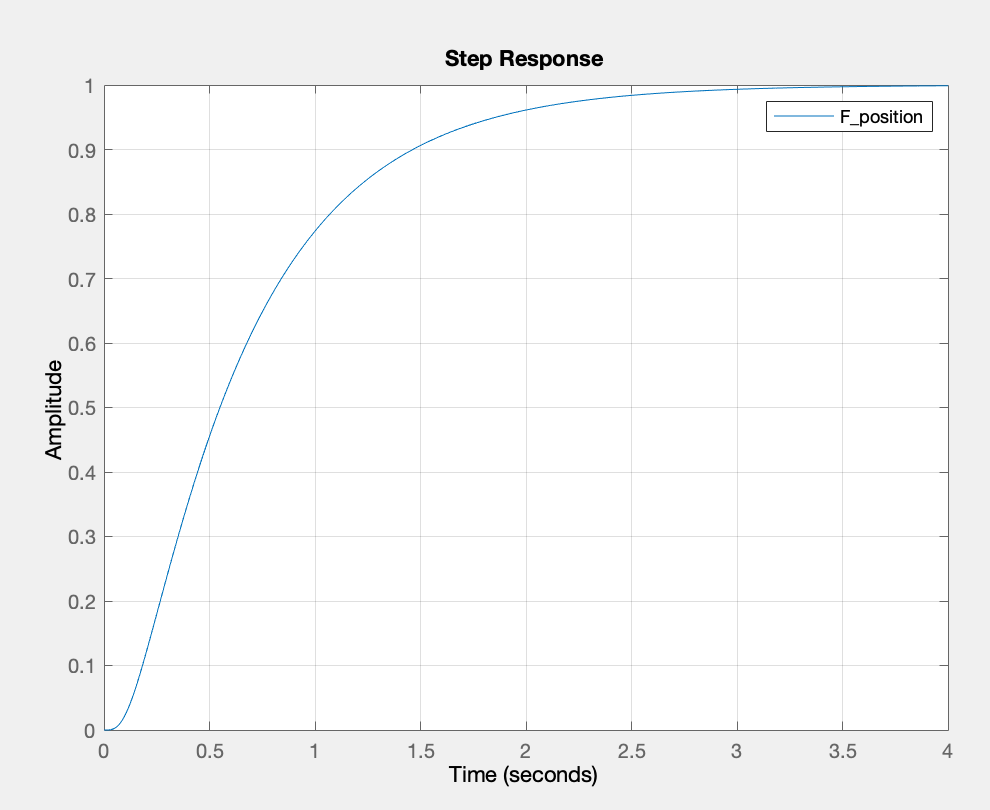
\includegraphics[width=\textwidth]{1_step1.4}
	\end{subfigure}
	\caption{Position control loop with  $wc_{p} $=1.4 rad/s}
	\label{fig:Bode and Step P 1.4}
\end{figure*}

On the other hand, we can accept even a ratio between the speed cutting frequency and the position one up to 25 \%. In this scenario we can fix the proportional gain in order to have a bandwidth around 3 rad/s, and we can notice that the position loop is not so influenced by the inner one.


\begin{figure*}[h]
	\centering
	\begin{subfigure}{0.45\columnwidth}
		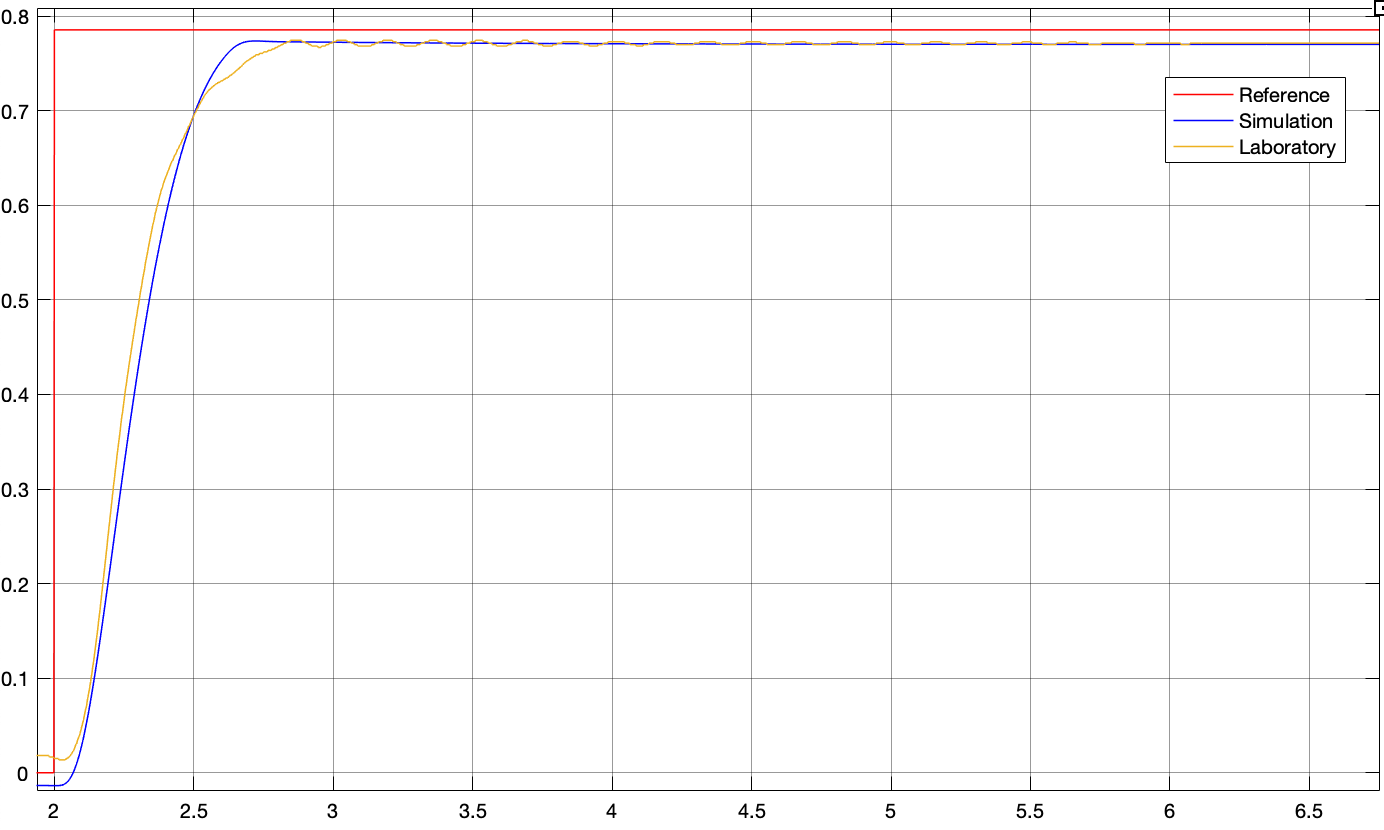
\includegraphics[scale=0.3]{pos_1_dof}
		\caption{Position}
	\end{subfigure}
	\begin{subfigure}{0.45\columnwidth}
		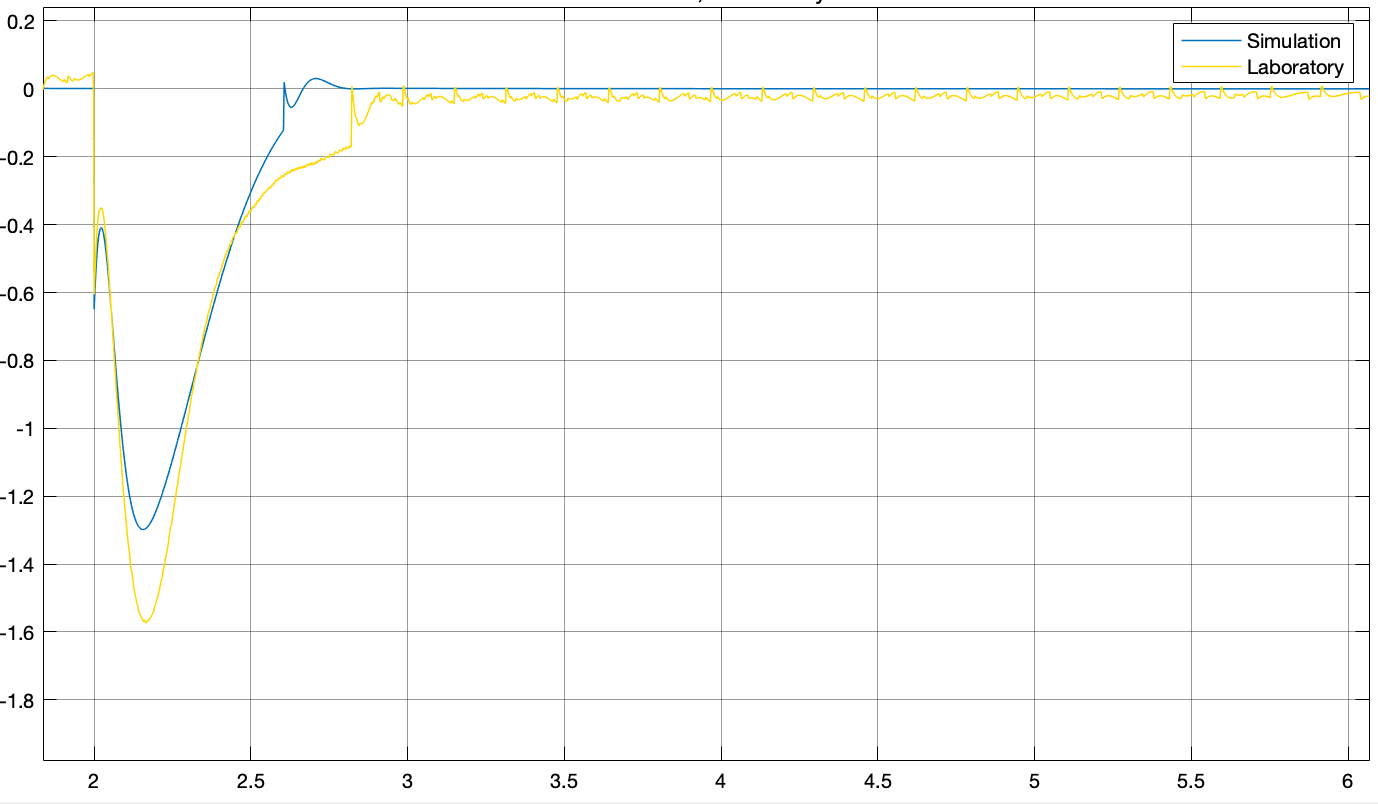
\includegraphics[scale=0.3]{volt_1_dof}
		\caption{Voltage}
	\end{subfigure}
	\caption{Step response with $k_{p} $=3.5}
	\label{fig:Pos_1dof_3.5}
\end{figure*}

Due to the friction, the position reached by the mass is not exactly the reference one. The controller integrates this small error and the control input raises slowly. Because the static friction coefficient is higher than the dynamic one, the load will move only after a few seconds, during which the controller has kept integrating the error asking for an increasing control action.
Once that the input is enough large to counteract the static friction, the load moves and the friction decreases, making the applied control input stronger than what needed. The result is that the load moves over the reference, generating an error that is even bigger than the original one.
For the above-mentioned reasons, we use a switch logic that deactivates the integrative action of the inner loop whenever the position error is smaller than a threshold equal to 0.85 degrees. On the other hand, we are not able to reach the reference since we use only the proportional action.

\begin{figure*}[h]
	\centering
	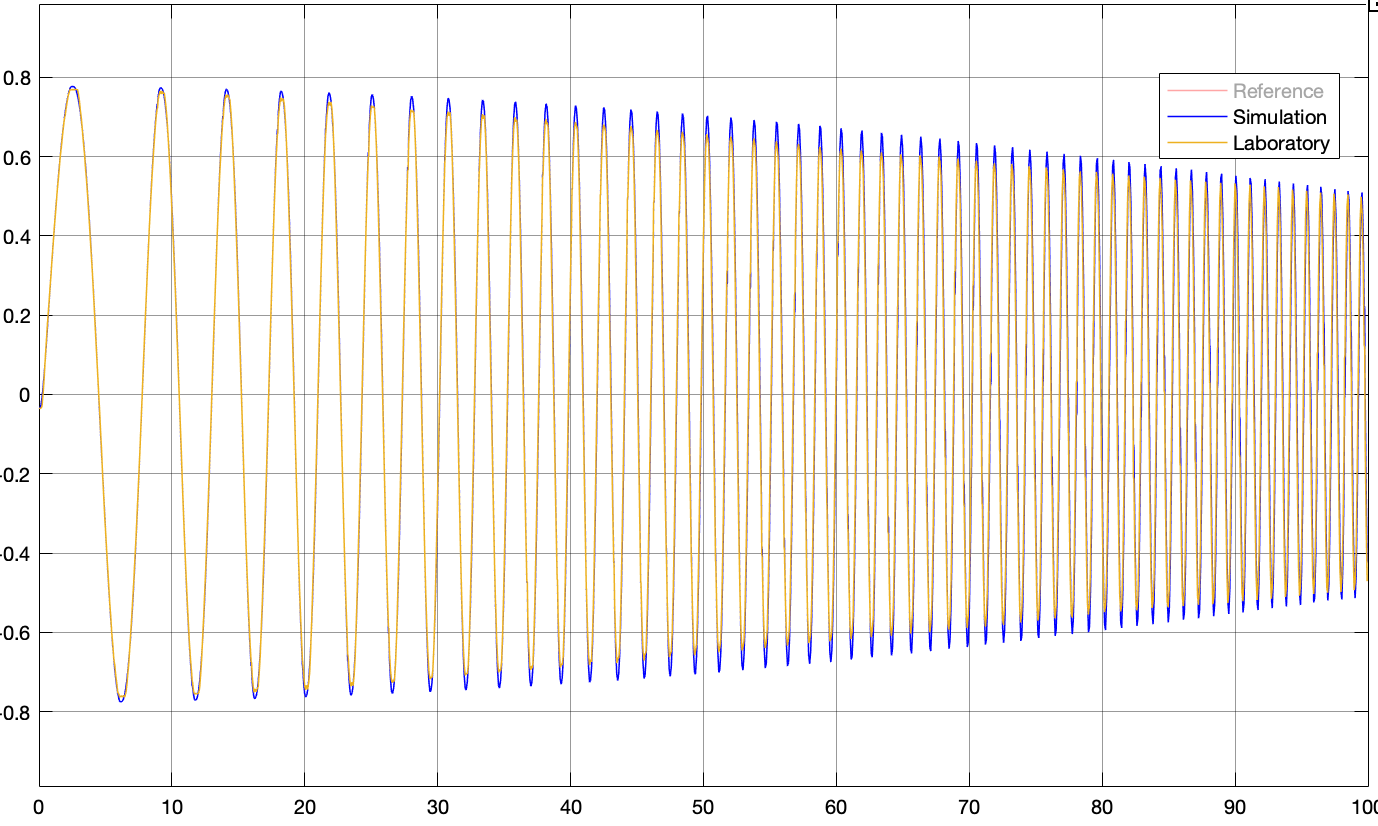
\includegraphics[scale=0.4]{sine_pos_1dof}
	\caption{Sinesweep experiment from 0.1 Hz to 1 Hz in 100s}
	\label{fig:sinesweep_pos_1dof}
\end{figure*}

Also in this case, we use sinewseep experiment to estimate the bandwidth of the closed loop system. We can observe that the simulation and laboratory data are really close and the cutting frequency is around 5.5 rad/s for the simulated system and 4.5 rad/s for the real system.

\newpage
\section{2-DOF System}
We consider as transfer function from voltage to the second mass speed:\\
\\
\[	
G(s)=
\frac{-1.244*10^{8}}{s^5+40.9*s^{4}+4833*s^{3}+1.686*10^{5}*s^{3}+3.327*10^{6}*s+7.355*10^{7}}
\]
\\



\begin{figure*}[h]
	\centering
	\begin{subfigure}{0.4\columnwidth}
		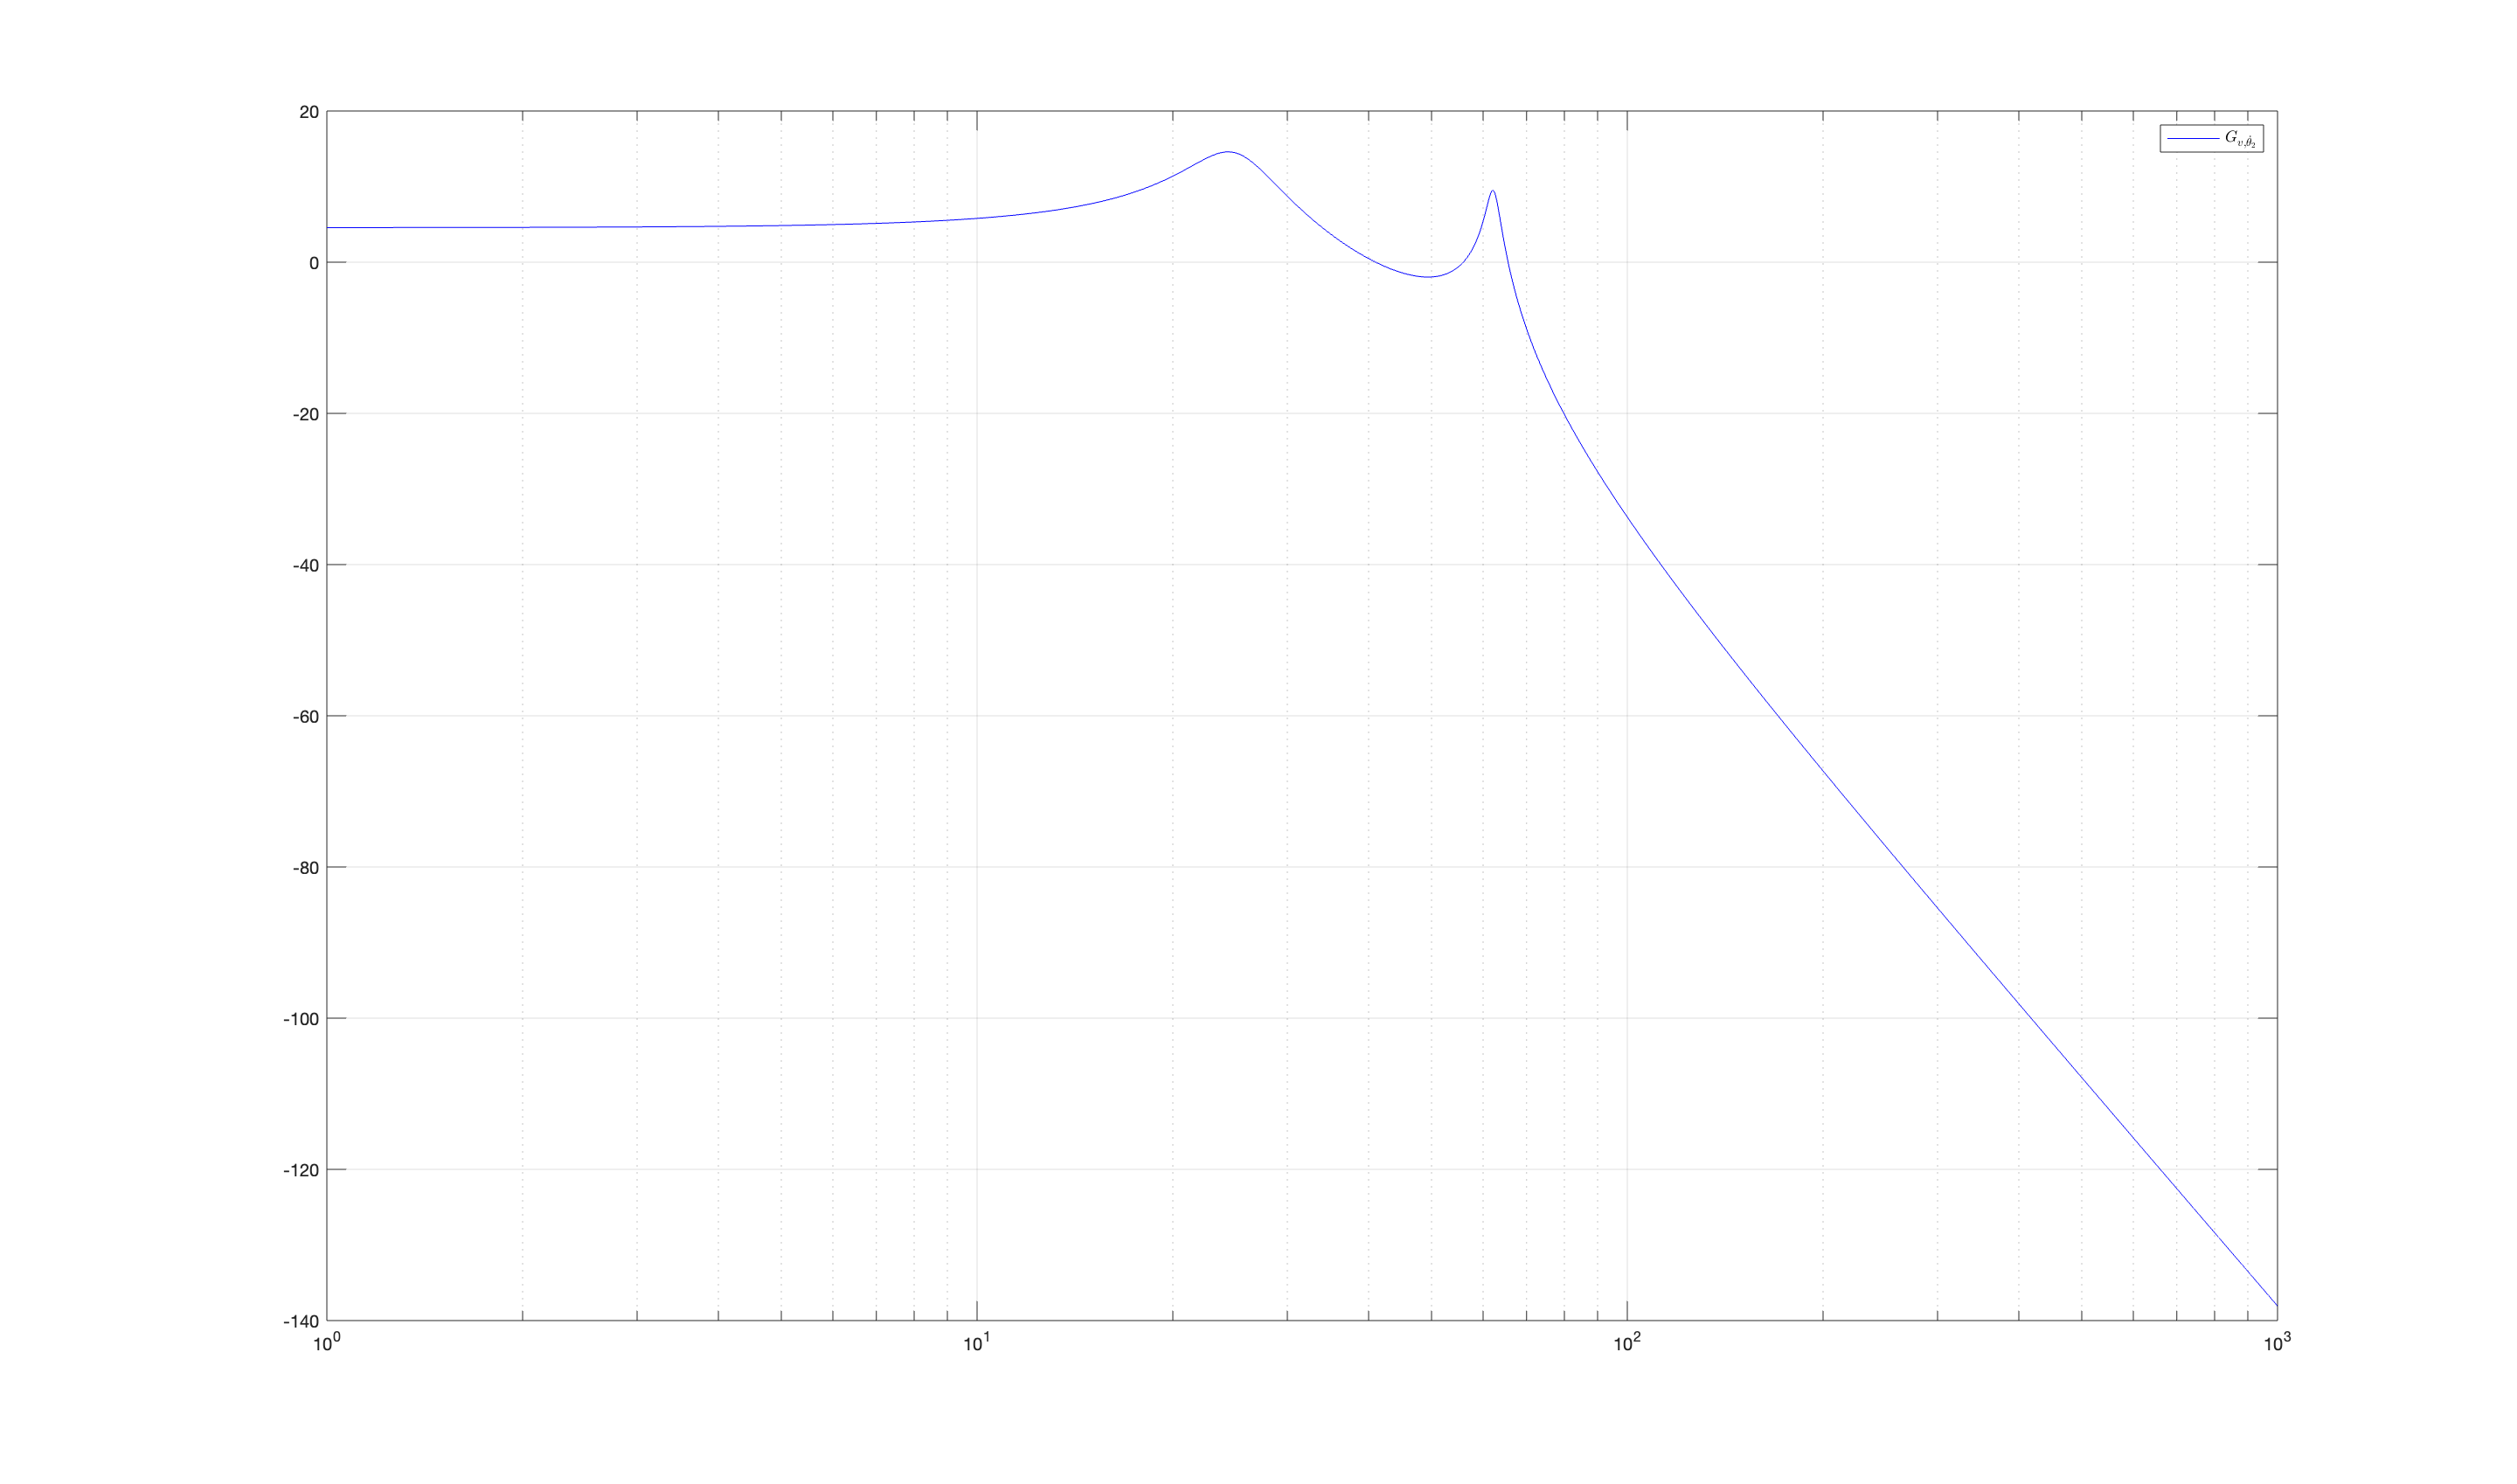
\includegraphics[width=\textwidth]{1_bodeG2}
	\end{subfigure}
	\begin{subfigure}{0.4\columnwidth}
		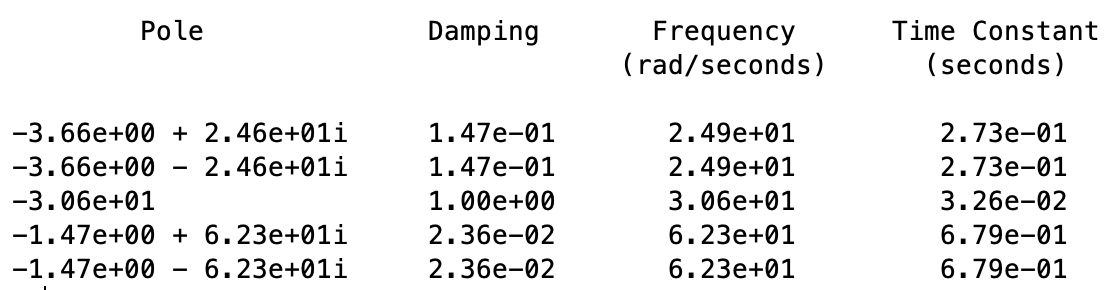
\includegraphics[width=\textwidth]{1_poleG2}
	\end{subfigure}
	\caption{G(s)}
	\label{fig:G(s)2dof}
\end{figure*}

As it is possible to notice in figure \ref{fig:G(s)2dof}, there is a couple of complex conjugated poles with low damping coefficient. We decide so to apply a notch filter, thanks to which we are able to delete these poles and substitute them with a couple of complex conjugated poles at frequency 100 rad/s and a damping coefficient equal to 0.72. The reason why we decide to postpone the poles frequency instead of using the original one is explain in the speed control loop section.


\begin{figure*}[h]
	\centering
	\begin{subfigure}{0.35\columnwidth}
		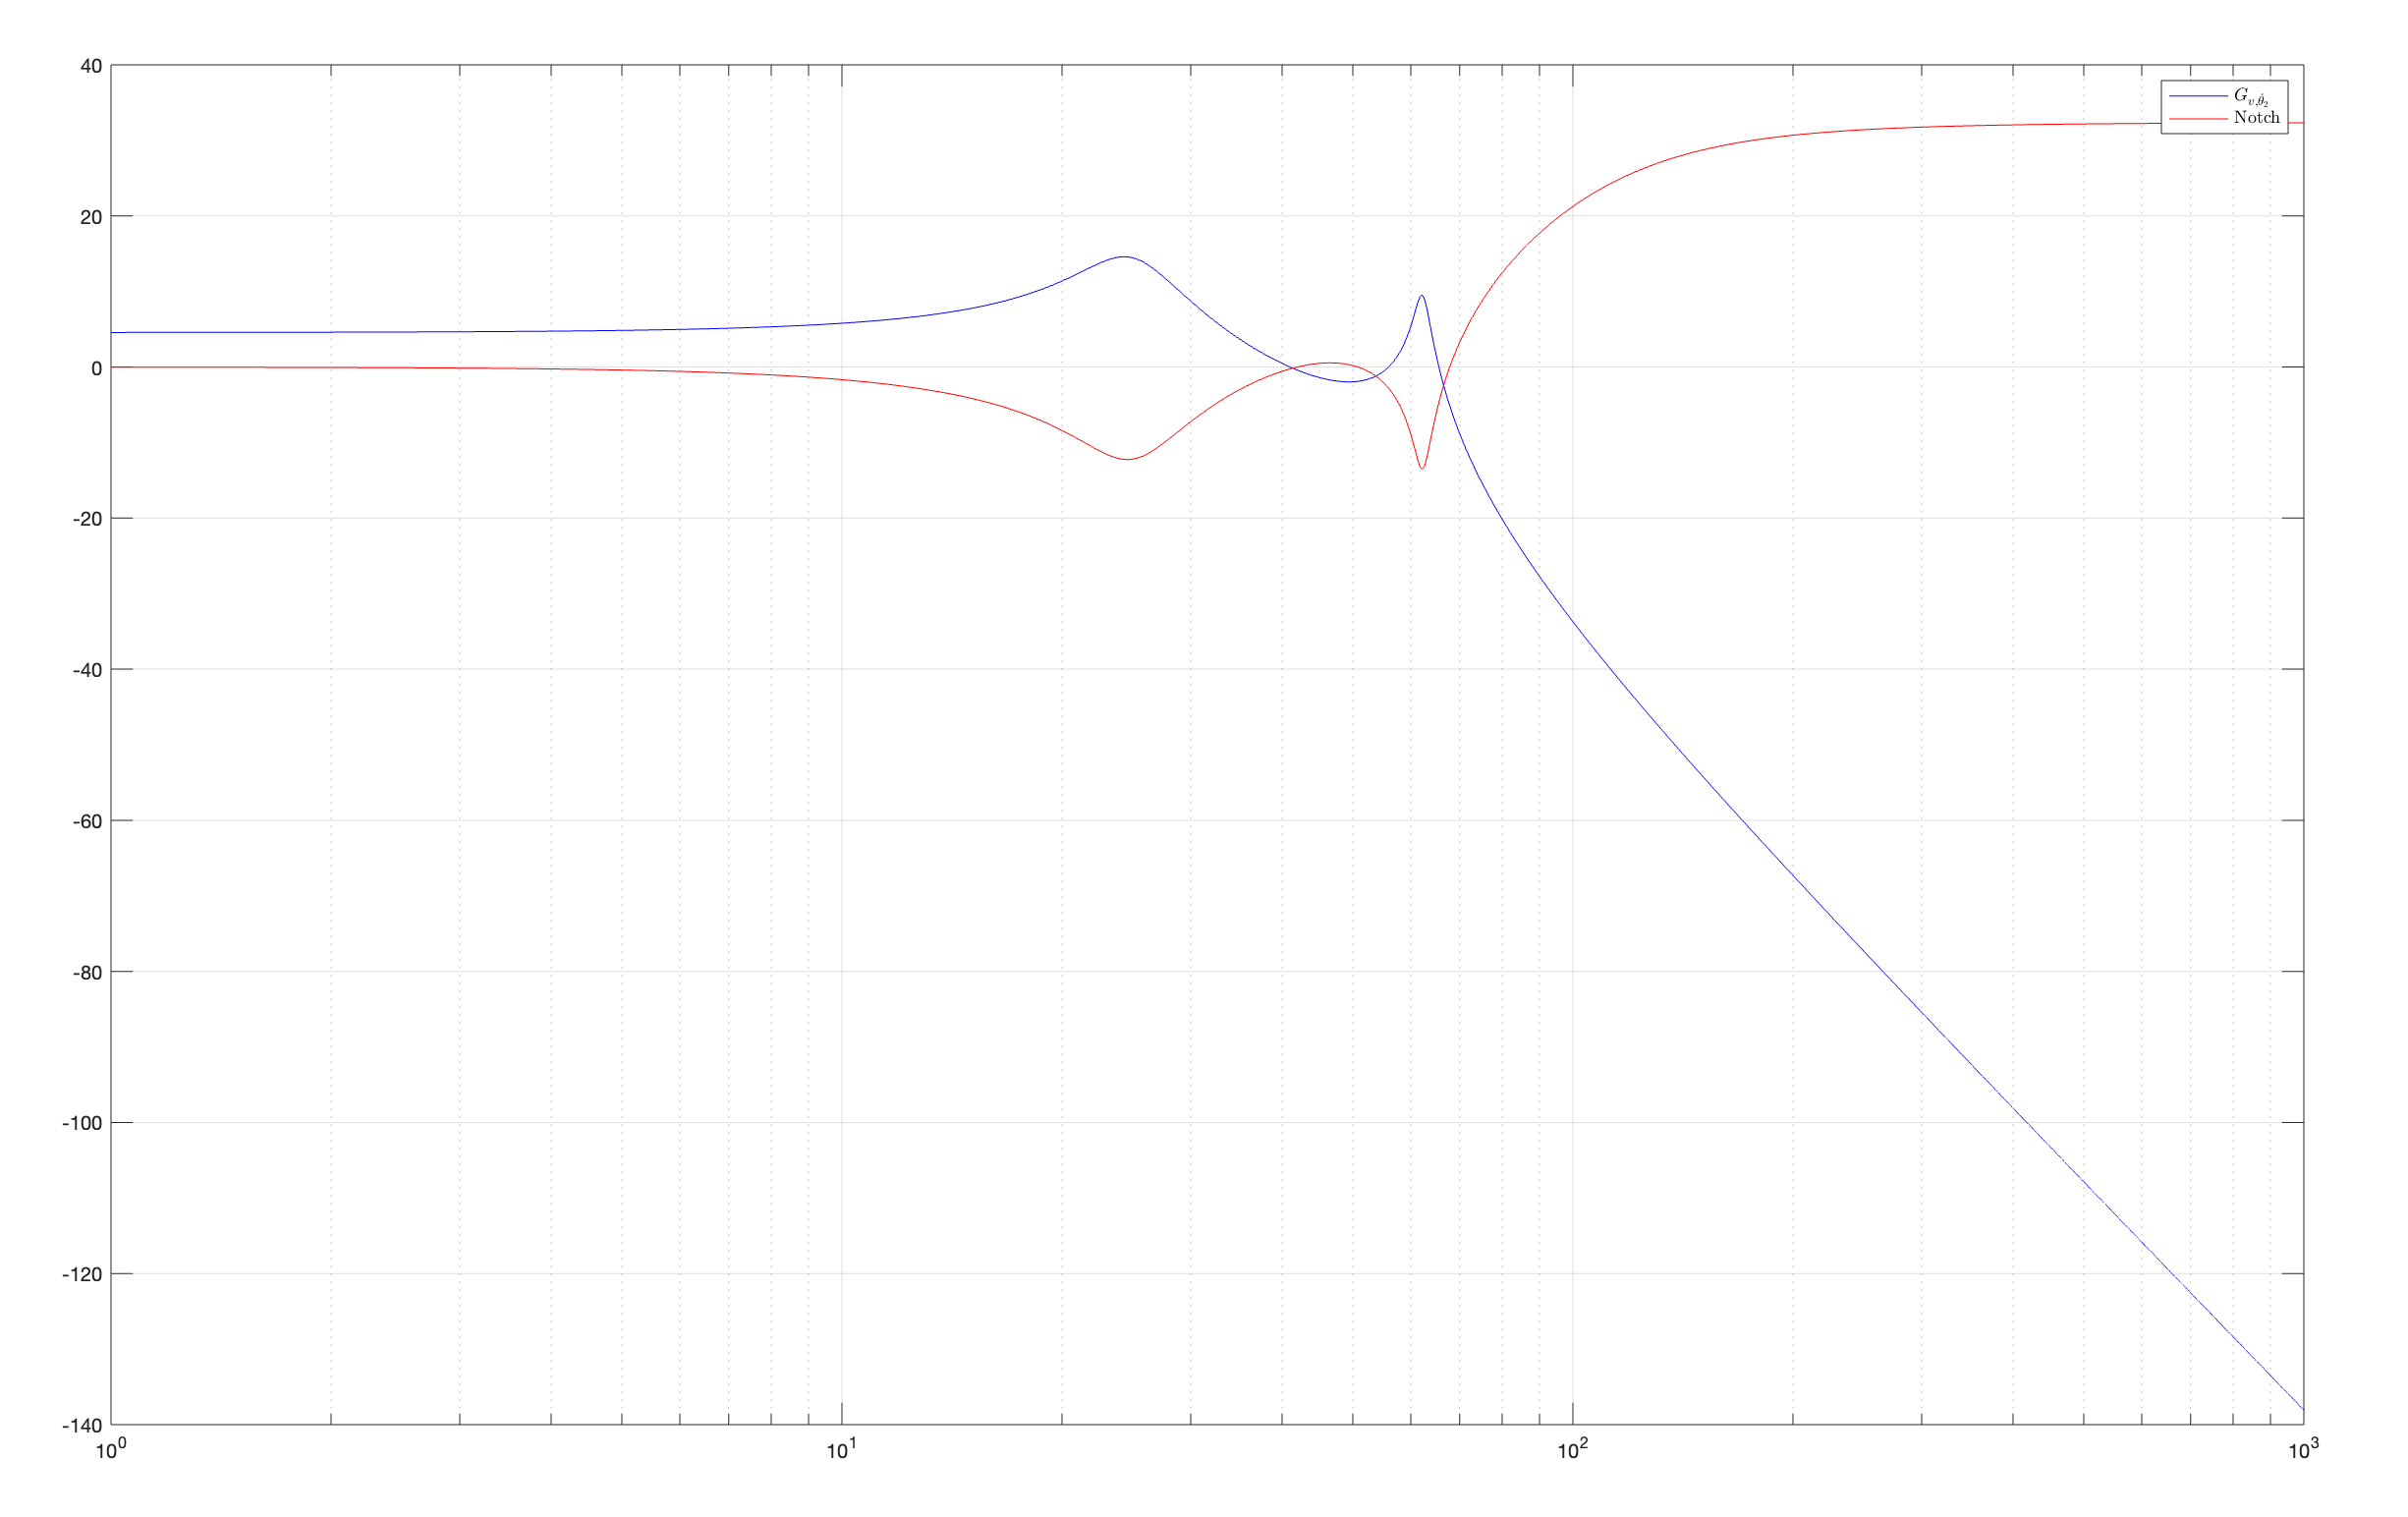
\includegraphics[width=\textwidth]{1Nf_G2}
		\subcaption{Nf(s) and G(s)}
	\end{subfigure}
	\begin{subfigure}{0.35\columnwidth}
		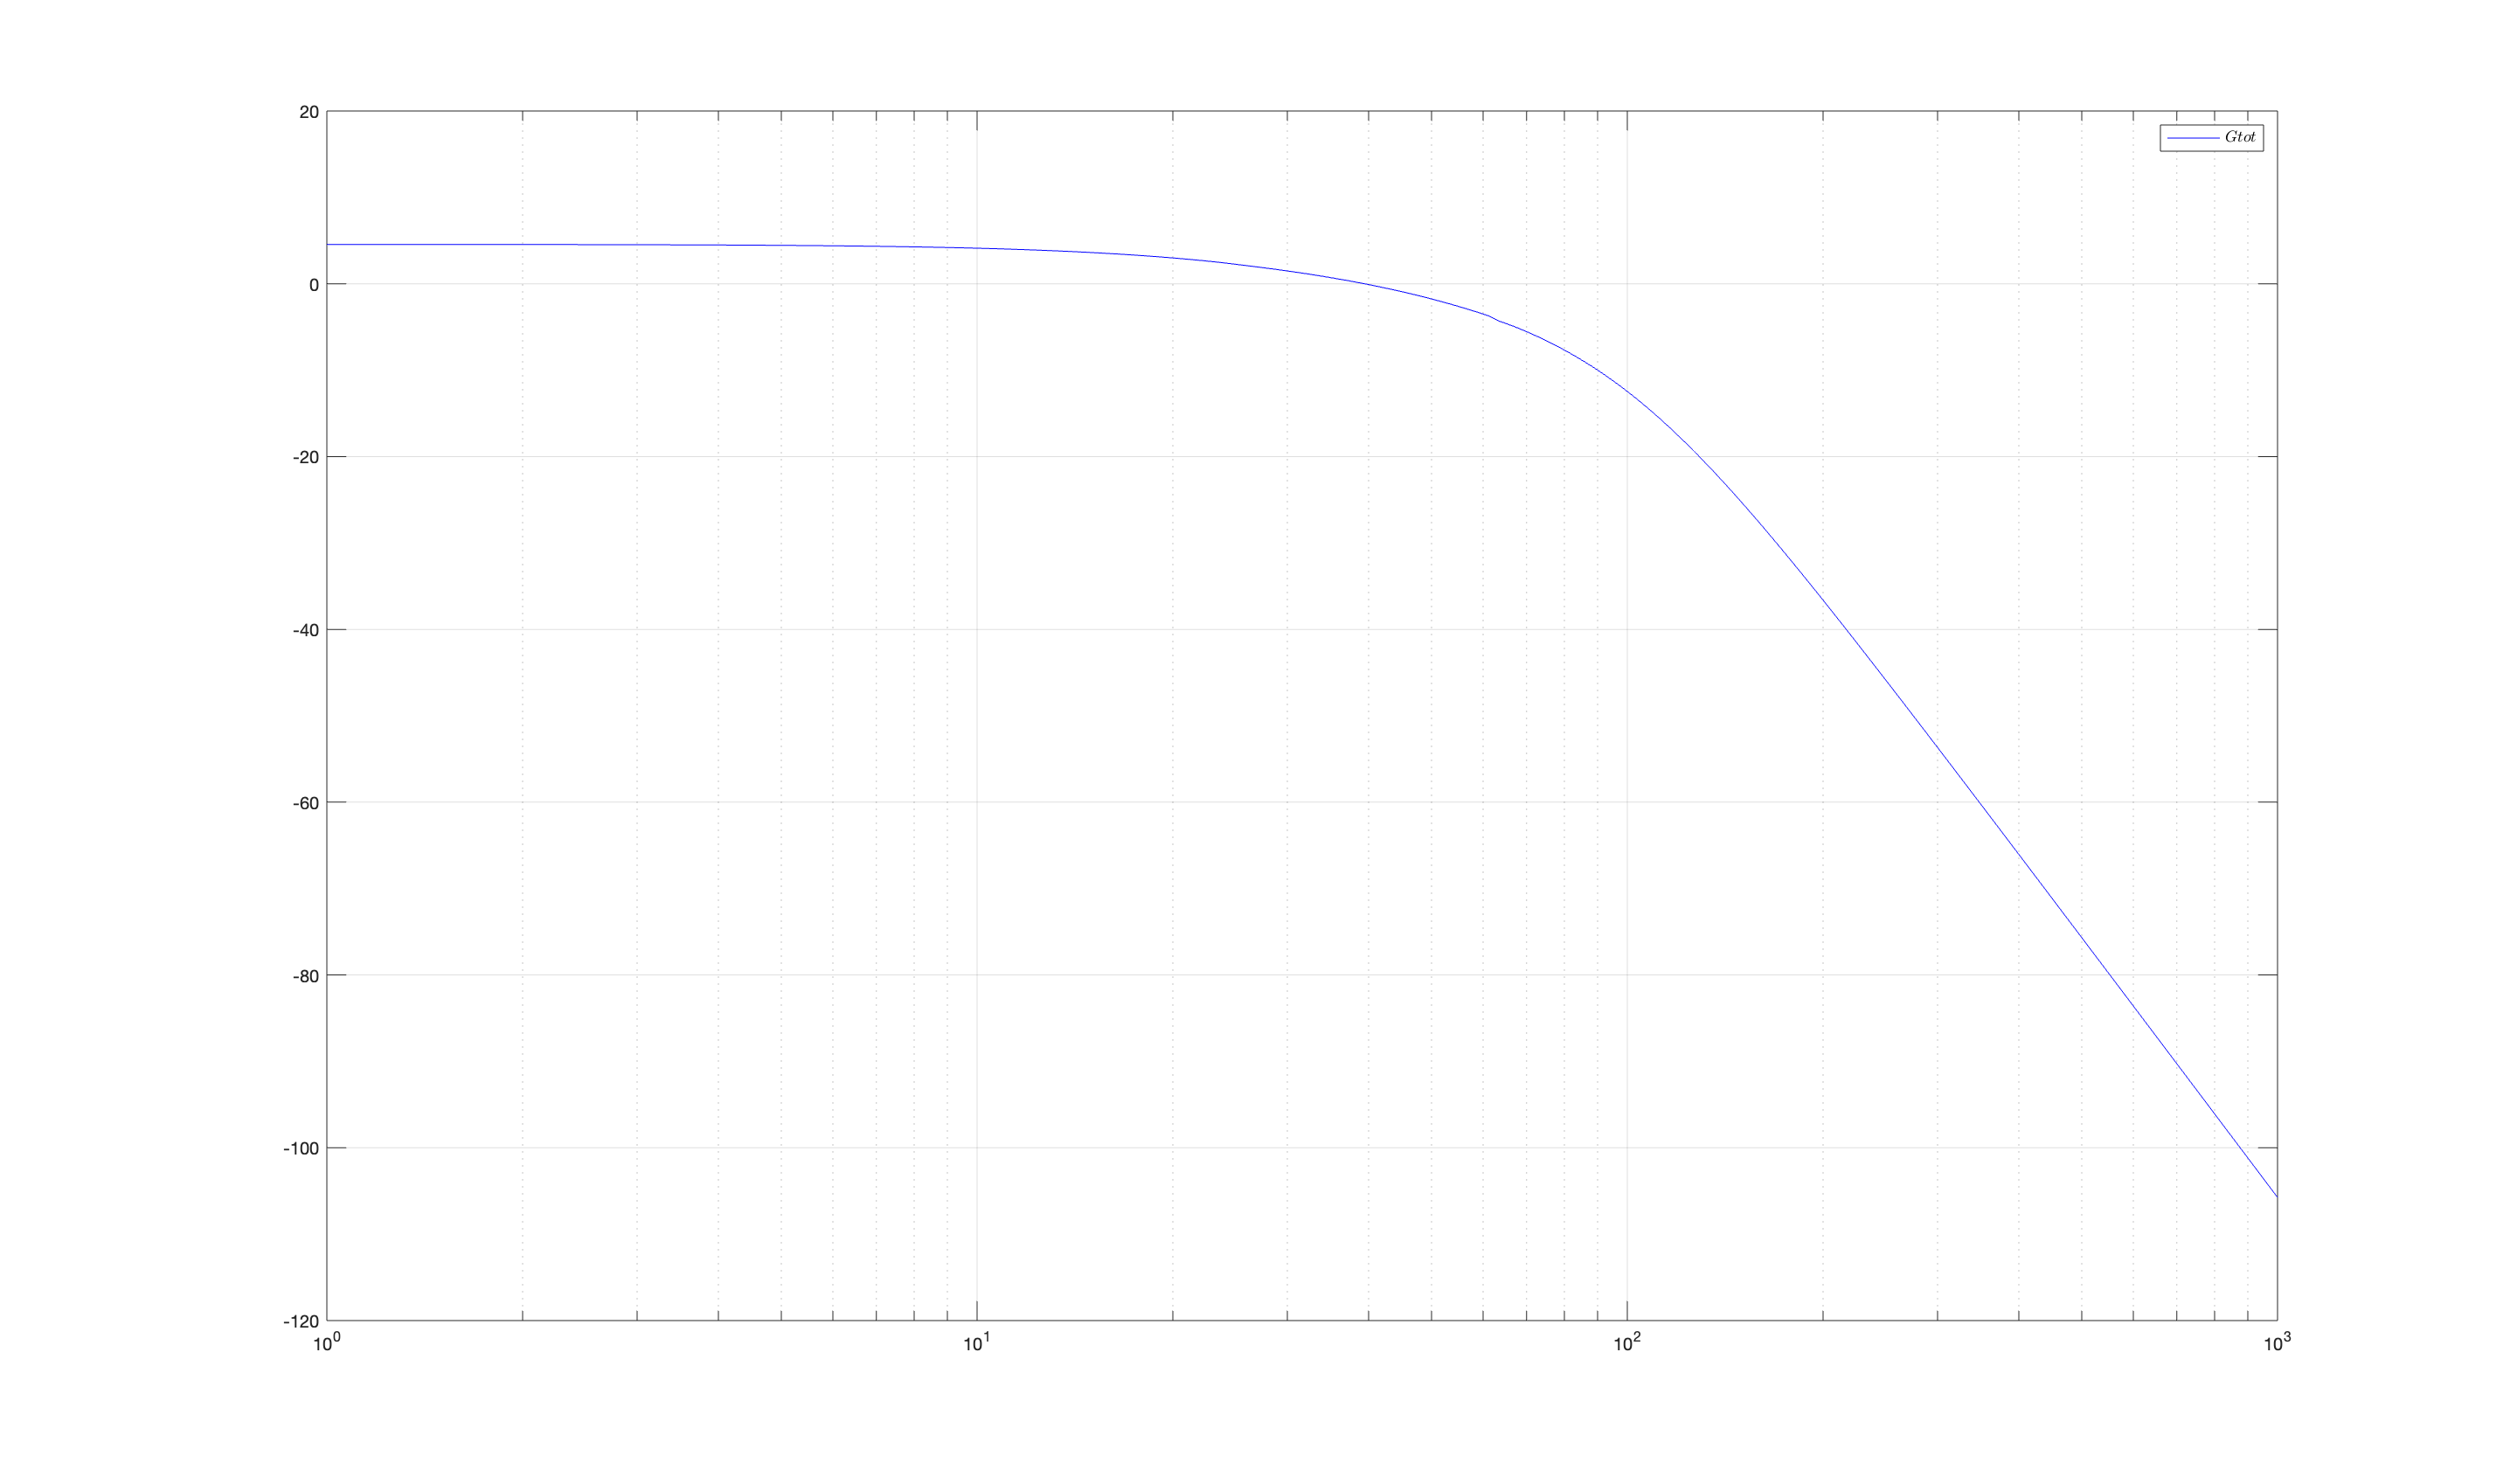
\includegraphics[width=\textwidth]{1_G2tot}
		\subcaption{$G_{tot}$(s)}
	\end{subfigure}
	\caption{Plant G(s) with Notch Filter Nf(s): $G_{tot}$(s)}
	\label{fig:Plant G(s)with Notch Filter2}
\end{figure*}


Applying the notch filter represented in figure \ref{fig:Plant G(s)with Notch Filter2}(a), we obtain the plant $G_{tot}$(s) of figure \ref{fig:Plant G(s)with Notch Filter2}(b) that is the one we are going to control.

\newpage 
\subsection{Speed Control Loop}
We use a PI-regulator enriched with an anti-wind-up structure; we decided then to cancel out the real pole at 30.6 rad/s.
\\
\[
R(s)=-wc_v
\frac{\frac{s}{30.6}+1}{s}
\]
\\
As in the 1-DOF scenario, the presence of the Notch Filter postpones the cutting frequency imposed by the PI, indeed the wcv written in the legends below, are referred to the same parameter written in R and not to the real bandwidth of the speed-loop.







